\documentclass[tese_patricia]{subfiles}% !TeX spellcheck = pt_BR

\begin{document}
\nomenclature[B,01]{$\domainT$}{Domínio computacional de um escoamento em um instante de tempo arbitrário $t$;}
\nomenclature[B,02]{$n_{sd}$}{Dimensão espacial;}
%\nomenclature[B,03]{$\boundaryT$}{Contorno do domínio computacional de um escoamento em um instante de tempo arbitrário $t$;}
%\nomenclature[B,04]{$t$}{Instante de tempo arbitrário;}
%\nomenclature[B,05]{$\totalTime$}{Intervalo de tempo total da análise;}
%\nomenclature[B,06]{$\density$}{Massa específica do fluido;}
%\nomenclature[B,07]{$\velocity$}{Campo de velocidades de um escoamento;}
%\nomenclature[B,08]{$\sbodyforce$}{Força de domínio em um escoamento;}
%\nomenclature[B,09]{$\stresstensor$}{Tensor das tensões de Cauchy;}
%\nomenclature[B,10]{$\press$}{Campo de pressões de um escoamento;}
%\nomenclature[B,11]{$\viscosity$}{Viscosidade dinâmica do fluido;}
%\nomenclature[B,12]{$\strainratetensor(\bullet)$}{Tensor taxa de deformação de um campo escalar ou vetorial;}
%\nomenclature[B,13]{$\mathbf{g}$}{Condições de contorno de Dirichlet;}
%\nomenclature[B,14]{$\mathbf{h}$}{Condições de contorno de Neumann;}
%\nomenclature[B,15]{$\left(\boundaryT\right)_{\mathbf{g}$}}{Porção do contorno com condições de contorno de Dirichlet;}
%\nomenclature[B,16]{$\left(\boundaryT\right)_{\mathbf{h}$}}{Porção do contorno com condições de contorno de Neumann;}
%\nomenclature[B,17]{$\normal$}{Vetor normal ao contorno do domínio computacional;}
%\nomenclature[B,18]{$\Omega_X$}{Domínio computacional inicial ou material;}
%\nomenclature[B,19]{$\mathbf{X}$}{Coordenadas no domínio inicial ou material de um ponto arbitrário;}
%\nomenclature[B,20]{$\Omega_x$}{Domínio computacional atual;}
%\nomenclature[B,21]{$\pos$}{Coordenadas atuais de um ponto arbitrário;}
%\nomenclature[B,22]{$\Omega_{\bar{x}}$}{Domínio computacional de referência;}
%\nomenclature[B,23]{$\posAle$}{Coordenadas de referência de um ponto arbitrário;}
%\nomenclature[B,24]{${\mathbf{\Phi}}$}{Função mudança de configuração do domínio computacional material para o domínio computacional atual;}
%\nomenclature[B,25]{$\bar{\mathbf{\Phi}}$}{Função mudança de configuração do domínio computacional de referência para o domínio computacional atual;}
%\nomenclature[B,26]{$\velocityALE$}{Velocidade dos pontos de referência;}
%\nomenclature[B,27]{$\usolution$}{Espaço vetorial das funções aproximadoras do campo de velocidades;}
%\nomenclature[B,28]{$\psolution$}{Espaço vetorial das funções aproximadoras do campo de pressões;}
%\nomenclature[B,29]{$\uweighting$}{Espaço vetorial das funções ponderadoras do campo de velocidades;}
%\nomenclature[B,30]{$\pweighting$}{Espaço vetorial das funções ponderadoras do campo de pressões;}
%\nomenclature[B,31]{$\utest$}{Função ponderadora pertencente ao espaço $\uweighting$;}
%\nomenclature[B,32]{$\ptest$}{Função ponderadora pertencente ao espaço $\pweighting$;}
%\nomenclature[B,33]{$(\bullet)^h$}{O superscrito $h$ indica, em todos os casos, a discretização em elementos finitos da variável;}
%\nomenclature[B,34]{$\domain^{e}$}{Domínio computacional de um elemento finito;}
%\nomenclature[B,35]{$\nel$}{Número de subdomínios do domínio discreto;}
%\nomenclature[B,36]{$N_nos$}{Número de nós ou pontos de controle do domínio discreto;}
%\nomenclature[B,37]{$N$}{Função de forma da discretização do domínio;}
%\nomenclature[B,38]{$(\bullet)_A$}{O subscrito $A$ indica, em todos os casos, que se trata da variável respectiva ao nó $A$ da malha de elementos finitos;}
%\nomenclature[B,39]{$\SUPG$}{Parâmetro de estabilização do método \textit{Streamline-Upwind/Petrov-Galerkin} (SUPG);}
%\nomenclature[B,40]{$\PSPG$}{Parâmetro de estabilização do método \textit{Pressure-Stabilizing/Petrov-Galerkin} (PSPG);}
%\nomenclature[B,41]{$\LSIC$}{Parâmetro de estabilização do método \textit{Least-Squares on the Incompressibility Constraint} (LSIC);}
%\nomenclature[B,42]{$\resMom$}{Resíduo da equação da quantidade de movimento;}
%\nomenclature[B,43]{$\resPre$}{Resíduo da equação da continuidade;}
%\nomenclature[B,44]{$\NNSM$}{Resíduo do vetor discreto da equação da quantidade de movimento;}
%\nomenclature[B,45]{$\NNSC$}{Resíduo do vetor discreto da equação da continuidade;}
%\nomenclature[B,46]{$\Acceleration$}{Vetor nodal dos graus de liberdade respectivo a aceleração;}
%\nomenclature[B,47]{$\Velocity$}{Vetor nodal dos graus de liberdade respectivo a velocidade;}
%\nomenclature[B,48]{$\Press$}{Vetor nodal dos graus de liberdade respectivo a pressão;}
%\nomenclature[B,49]{$\matrixQ$}{Tensor métrico do elemento;}
%\nomenclature[B,50]{$\coordAdimen$}{Coordenadas adimensionais do elemento onde são definidas as funções de forma;}
%\nomenclature[B,51]{$\matrixD$}{Matriz que escalona o tensor métrico do elemento;}
%\nomenclature[B,52]{$\matrixQhat$}{Tensor métrico do elemento escalonado;}
%\nomenclature[B,53]{$\bar{\coordAdimen}$}{Coordenadas adimensionais do espaço preferido;}
%\nomenclature[B,54]{$\mathbf{C}$}{Tensor de transformação de Bezier;}
%\nomenclature[B,55]{$\RGN$}{Comprimento de escala do elemento finito;}
%\nomenclature[B,56]{$\rRGN$}{Vetor unitário no sentido da velocidade do fluido no elemento finito;}
%\nomenclature[B,57]{$\matrixG$}{Matriz auxiliar para o cálculo do comprimento direcional do elemento;}
%\nomenclature[B,58]{$h_{min}$}{Mínimo comprimento de escala do elemento finito;}
%\nomenclature[B,59]{$h_{max}$}{Máximo comprimento de escala do elemento finito;}
%\nomenclature[B,60]{$\SUGNi,\SUGNii,\SUGNiii$}{Parâmetros da estabilização SUPG/PSPG/LSIC correspondentes aos termos convectivos, inerciais e viscosos, respectivamente;}
%\nomenclature[B,61]{$\timeStep$}{sub-intervalo de tempo $t$;}
%\nomenclature[B,62]{$\rRGN_{reg}$}{Vetor unitário no sentido da velocidade do fluido modificado de maneira a evitar problemas numéricos devido divisão por zero;}
%\nomenclature[B,63]{$\varepsilon$}{Constante pequena utilizada no cálculo de $\rRGN_{reg}$;}
%\nomenclature[B,64]{$t_{n}$}{extremidade menor de tempo do sub-intervalo $\timeStep$;}
%\nomenclature[B,65]{$t_{n+1}$}{extremidade maior de tempo do sub-intervalo $\timeStep$;}
%\nomenclature[B,66]{$\alpham, \alphaf, \gamma$}{Parâmetros reais do esquema de integração temporal $\alpha$-generalizado;}
%\nomenclature[B,67]{$\specRadius$}{Raio espectral da matriz de amplificação;}
%\nomenclature[B,68]{$\Reynolds$}{Número de Reynolds;}
%\nomenclature[B,69]{$\velocinfty$}{Velocidade de referência;}
%\nomenclature[B,70]{$L$}{Comprimento característico/de referência do escoamento;}
%\nomenclature[B,71]{$\kviscosity$}{Viscosidade cinemática do fluido;}
%\nomenclature[B,72]{$u_x$}{Velocidade do escoamento na direção $x$;}
%\nomenclature[B,73]{$u_y$}{Velocidade do escoamento na direção $y$;}
%\nomenclature[B,74]{$u_n$}{Velocidade do escoamento na direção normal ao contorno;}
%\nomenclature[B,75]{$F_L, F_D$}{Forças de sustentação e arrasto, respectivamente;}
%\nomenclature[B,76]{$C_L, C_D$}{Coeficiente de sustentação e arrasto, respectivamente;}
%\nomenclature[B,77]{$\Strouhal$}{Número de Strouhal;}
%\nomenclature[B,78]{$f_V$}{Frequência de desprendimento dos vórtices;}

% ---------------------------------------------------------- 
% Métodos de \part{\part{malhas}} sobrepostas
% ----------------------------------------------------------
\chapter[Dinâmica dos fluidos computacional]{Dinâmica dos fluidos computacional}
\label{capitulo:Cap2}
% ----------------------------------------------------------

O escoamento isotérmico de um fluido newtoniano é descrito pelas equações advindas da conservação da quantidade de movimento, ou de Navier-Stokes, e da conservação de massa. Nos casos em que ocorram variações significativas no campo de temperatura, ou em escoamentos compressíveis, a equação da conservação de energia deve ser adicionada ao sistema. Essas equações governantes, juntamente com as relações constitutivas, resultam em um sistema de equações diferenciais não lineares que descrevem o comportamento do escoamento no tempo e no espaço. 

Neste trabalho, são investigados escoamentos incompressíveis, isotérmicos e com contornos móveis. As seções seguintes apresentam a abordagem adotada para a resolução desse tipo de problema, bem como sua implementação computacional. Utiliza-se uma formulação Arbitrária Euleriana-Lagrangiana (ALE) para representar as equações, e a discretização espacial é realizada por meio do método dos elementos finitos (FEM) ou da análise isogeométrica (IGA).

Para tratar questões numéricas recorrentes nesse sistema de equações, como as oscilações espúrias em casos de convecção dominante, típicas da aplicação do método dos resíduos ponderados baseado na formulação clássica de Galerkin, emprega-se a metodologia SUPG. Adicionalmente, a estabilização PSPG é aplicada com o objetivo de contornar a condição imposta pelo critério de \textit{Ladyzhenskaya-Babuška-Brezzi} (LBB). A integração no tempo é conduzida por meio do método $\alpha$-generalizado.

Ao final deste capítulo, é apresentado um algoritmo que detalha o esquema computacional de solução dos problemas da DFC, seguido pela resolução de alguns casos clássicos, utilizados como verificação da metodologia proposta.


\section{Equações governantes na descrição Euleriana} 


\subsection{Equação da conservação da massa}


Considere um volume de controle infinitesimal fixo no espaço, permeável a matéria e submetido a uma escoamento de velocidade $\velocity$, com componentes $u_1, u_2$, e $u_3$ (conforme fig. \ref{fig:VolInfi}).Para um intervalo de tempo infinitesimal $dt$, a lei da conservação da massa impõe que a variação de massa dentro do volume de controle seja igual ao fluxo líquido de massa que atravessa suas fronteiras, que pode ser expresso matematicamente da seguinte forma:

\begin{figure}[htb!]
	\centering 
	%\vspace{-1em} % Diminui o espaço antes da figura
	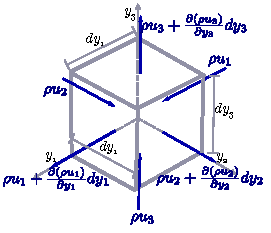
\includegraphics[scale=1.5,trim=0cm 0.0cm 0cm 0.0cm, clip=true]{Imagens/Cap2/conserMassa.pdf}	
	\caption{Volume de controle infinitesimal: Fluxo de massa}
	\label{fig:VolInfi}
	%\vspace{-1em} % Diminui o espaço antes da figura
\end{figure}


\begin{align}
	\begin{split}
	\frac{\partial \density}{\partial t}dV =& \left(\density u_1 dA_{1}  +  \density u_2 dA_{2} + \density u_3  dA_{3} \right) - \\  &\left(\left(\rho u_1 + \frac{\partial \rho u_1}{\partial y_1}dy_1 \right)dA_{1} + \left(\rho u_2+ \frac{\partial \rho u_2}{\partial y_2}dy_2 \right) dA_{2} + \left(\rho u_3 + \frac{\partial \rho u_3}{\partial y_3}dy_3 \right) dA_{3}\right), \label{eq:conserMassa1} 
	\end{split}
\end{align}

\noindent com $\density$ a massa específica do fluido e $dA_{i}$ a área referente à face ortogonal ao eixo $y_i$. Considerando que $dV = dy_1dA_1 = dy_2dA_2 = dy_3dA_3 $  e manipulando-se algebricamente a Eq. \ref{eq:conserMassa1} chega-se a seguinte expressão:

\begin{align}
	\frac{\partial \density}{\partial t} = - \frac{\partial \density u_{1}}{\partial y_1} - \frac{\partial \density u_{2}}{\partial y_2}- \frac{\partial \density u_{3}}{\partial y_3}.
	\label{eq:conserMassa} 
\end{align}

Para escoamentos incompressíveis, quando $\density$ é constante ao longo do tempo, a equação fica reduzida a:

\begin{align}
	 \frac{\partial u_{1}}{\partial y_1} + \frac{\partial u_{2}}{\partial y_2} + \frac{\partial u_{3}}{\partial y_3} = 0, 
\end{align} 

\noindent ou ainda:

\begin{align}
	\nabla_y \cdot \velocity = 0.
	\label{eq:conserMassaIncom} 
\end{align} 

\subsection{Equação da quantidade de movimento}


Para um volume de controle infinitesimal, a lei da conservação da quantidade de movimento afirma que a variação temporal da quantidade de movimento no interior do volume é determinada pela diferença entre o fluxo de quantidade de movimento que entra e o que sai pelas suas fronteiras, somada à resultante das forças aplicadas sobre o volume de controle.

Para chegar-se à equação da quantidade de movimento em sua forma conservativa partindo desse princípio, inicia-se com a avaliação das forças que atuam sobre um volume de controle infinitesimal no instante atual. Considerando o equilíbrio das forças externas e internas na direção $y_1$, de acordo o volume apresentado na Fig. \ref{fig:VolInfiFor}, chega-se na seguinte relação:


\begin{align}
	\begin{split}
	F_1 =& -\left(\sigma_{11}dy_2dy_3 + \sigma_{12}dy_1dy_3 + \sigma_{13}dy_1dy_2\right) + \\ & \left(\left(\sigma_{11} + \frac{\partial \sigma_{11}}{\partial y_1}dy_1 \right)dy_2dy_3 + \left(\sigma_{12}+ \frac{\partial \sigma_{12}}{\partial y_2}dy_2\right)dy_1dy_3 + \left(\sigma_{13}+ \frac{\partial \sigma_{13}}{\partial y_3}dy_3\right)dy_1dy_2\right) + \\& b_{1}dy_1dy_2dy_3, \label{eq:ResultFor} 
	\end{split}
\end{align}	

\noindent onde $F_1$ representa a resultante das forças externas na direção $y_1$; $\sigma_{ij}$ são as componentes $ij$ do tensor de tensões Cauchy ($\cauchyStress$); e $b_1$ representa a componente na direção $y_1$ do vetor força de campo por unidade de volume $\ebodyLoad$. Dividindo-se Eq. \ref{eq:ResultFor} por $dV$ e efetuando as subtrações, têm-se a força resultante por unidade de volume ($q_1$) dada por:

\begin{align}
		q_1 =\frac{\partial \sigma_{11}}{\partial y_1} + \frac{\partial \sigma_{12}}{\partial y_2} + \frac{\partial \sigma_{13}}{\partial y_3} + b_{1}.\label{eq:ForçasIntx1} 
\end{align}	

\begin{figure}[htb!]
	\centering 
	%\vspace{-1em} % Diminui o espaço antes da figura
	\includegraphics[scale=1.5,trim=0cm 0.0cm 0cm 0.0cm, clip=true]{Imagens/Cap2/tensão.pdf}	
	\caption{Volume de controle infinitesimal: Componentes de tensão e força na direção $y_1$}
	\label{fig:VolInfiFor}
	%\vspace{-1em} % Diminui o espaço antes da figura
\end{figure}

Considerando-se o equilíbrio das forças nas direções $y_2$ e $y_3$, pode-se escrever também:

\begin{align}
	q_2 =\frac{\partial \sigma_{21}}{\partial y_1} + \frac{\partial \sigma_{22}}{\partial y_2} + \frac{\partial \sigma_{23}}{\partial y_3} + b_{2}\label{eq:ForçasIntx2},
\end{align}	

\begin{align}
	q_3 =\frac{\partial \sigma_{31}}{\partial y_1} + \frac{\partial \sigma_{32}}{\partial y_2} + \frac{\partial \sigma_{33}}{\partial y_3} + b_{3}\label{eq:ForçasIntx3},
\end{align}

\noindent ou ainda:

\begin{align}
	\mathbf{q} = \mathbf{\nabla_y} \cdot \cauchyStress + \ebodyLoad.
\end{align}


Realizando-se o balanço da quantidade de movimento no volume de controle infinitesimal da Fig. \ref{fig:VolInfiQtdeMov}, e aplicando-se a lei da conservação da quantidade de movimento, pode-se chegar a seguinte equação:


\begin{align}
	\begin{split}
	\frac{\partial \density \velocity}{\partial t}dV =& u_1\density \velocity dA_1 + u_2\density \velocity dA_2 + u_3 \density \velocity dA_3 - \\
	 & \left(\left(u_1 \density \velocity + \frac{\partial u_1 \density \velocity}{\partial y_1}dy_1 \right)dA_1 + \left(u_2 \density \velocity + \frac{\partial u_2 \density \velocity}{\partial y_2}dy_2 \right)dA_2 \right. + \\ & \left.   \left(u_3 \density \velocity + \frac{\partial u_3 \density \velocity}{\partial y_3}dy_3 \right)dA_3\right) + \mathbf{q} dV,
	\label{eq:QtdeMov0} 
	\end{split}
\end{align}	

\noindent dividindo-se a Eq. \ref{eq:QtdeMov0} por $dV$ e efetuando-se as subtrações, chega-se a:

\begin{align}
		\frac{\partial \density \velocity}{\partial t} = 
		-\frac{\partial u_1 \density \velocity}{\partial y_1} 
		-\frac{\partial u_2 \density \velocity}{\partial y_2}  
		-\frac{\partial u_3 \density \velocity}{\partial y_3} + \mathbf{q},
		\label{eq:QtdeMov1} 
\end{align}

ou ainda:

\begin{align}
	\density\left(\frac{\partial\velocity}{\partial t} + \nabla_y \cdot \left(\velocity\otimes\velocity\right) - \sbodyforce \right) - \nabla_y \cdot \stresstensor  &= \mathbf{0}, \label{eq:QtdeMov2} 
\end{align}

\noindent com $\sbodyforce = \density \ebodyLoad$ que representa a força de campo por unidade de massa.

\begin{figure}[htb!]
	\centering 
	%\vspace{-1em} % Diminui o espaço antes da figura
	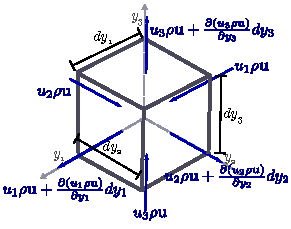
\includegraphics[scale=1.5,trim=0cm 0.0cm 0cm 0.0cm, clip=true]{Imagens/Cap2/conserQtdeMov.pdf}	
	\caption{Volume de controle infinitesimal: Fluxo de quantidade de Movimento}
	\label{fig:VolInfiQtdeMov}
	%\vspace{-1em} % Diminui o espaço antes da figura
\end{figure}

Da consideração da equação da continuidade, a Eq. \ref{eq:QtdeMov2} pode ser rescrita ainda em sua forma convectiva como:

\begin{align}
	\density\left(\frac{\partial\velocity}{\partial t} + \left( \velocity \cdot \nabla_y \right)  \velocity  - \sbodyforce \right) - \nabla_y \cdot \stresstensor = \mathbf{0}. \label{eq:Navier-Stokes} 
\end{align}

O tensor de tensões de Cauchy $\stresstensor$ é definido para fluidos newtonianos incompressíveis pela seguinte relação constitutiva:

\begin{align}
\stresstensor &= -p\unittensor + 2\viscosity\straintensor(\velocity),\label{eq:StressTensor}
\end{align}

\noindent onde $p$ representa a pressão, $\viscosity$ a viscosidade dinâmica do fluido e $\straintensor$ é o tensor taxa de deformação, definido como:


\begin{align}
\straintensor\left(\velocity\right) = \frac{1}{2}\left(\nabla_y\velocity + \nabla_y\velocity^{T}\right). 
\label{eq:StrainTensor}
\end{align}

\subsection{Formulação forte da mecânica dos fluidos}

Seja $\domain \in \realspace^{nsd}$, com $\nsd = 2,3$, o domínio espacial que define o escoamento do fluido com contorno $\boundary = \boundary_D \cup \boundary_N$, no instante $t \in (0,T)$ (ver Fig. \ref{fig:DomFluid}).

Para escoamentos incompressíveis isotérmicos o fluido possui movimento descrito pela equação da quantidade de movimento, ou equações de Navier-Stokes (Eq. \ref{eq:Navier-Stokes}) e da conservação de massa (Eq. \ref{eq:conserMassaIncom}). Para completar a formulação da mecânica dos fluidos, condições de contorno devem ser especificadas. Em geral, em uma dada parte do contorno espacial, condições de contorno essenciais (Dirichlet) ou naturais (Neumann) são aplicadas. Dessa forma, o escoamento é governado pelo seguinte conjunto de equações:

\begin{equation}
	\left\{
	\begin{array}{l}
		\density\left(\frac{\partial\velocity}{\partial t} + \velocity\cdot\nabla_y\velocity - \sbodyforce \right) - \nabla_y \cdot \stresstensor = \mathbf{0} \ \textrm{em} \ \domain\\
		\nabla_y \cdot \velocity = 0 \ \textrm{em} \ \domain\\
		\velocity = \velocityD \ \textrm{em} \ \GammaD \\
		\stresstensor \cdot \snormal = \surfaceLoad \ \textrm{em} \ \GammaN,
	\end{array} \label{eq:ConjDFC}
	\right.
\end{equation}

\noindent sendo $\GammaD$ a porção do contorno com condições de contorno de Dirichlet, representadas pelo campo de velocidades $\velocityD$, e $\GammaN$ aquela com condições de contorno de Neumann, descritas pelas forças de superfície $\mathbf{h}$. A variável $\snormal$ representa o vetor unitário normal ao contorno $\Gamma_{N}$.

\begin{figure}[htb!]
	\centering 
	%\vspace{-1em} % Diminui o espaço antes da figura
	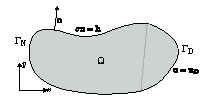
\includegraphics[scale=3.0,trim=0cm 0.0cm 0cm 0.0cm, clip=true]{Imagens/Cap2/dominiofluido.pdf}	
	\caption{Domínio para o problema da dinâmica dos fluidos computacional}
	\label{fig:DomFluid}
	%\vspace{-1em} % Diminui o espaço antes da figura
\end{figure}

\section{Descrição Euleriana-Lagrangiana arbitrária (ALE)} \label{Capítulo2:ALE}

A descrição Lagrangiana-Euleriana arbitrária \cite{DoneaGH:1982} representa uma generalização da descrição puramente Lagrangiana e da descrição puramente Euleriana do movimento do contínuo. A descrição Lagrangiana fixa a atenção em pontos materiais do contínuo, enquanto que na descrição Euleriana considera-se uma porção fixa do espaço ocupada pelo contínuo, e analisam-se os pontos materiais que passam por essa porção ao longo do tempo. Como consequência, na descrição puramente Lagrangiana a malha computacional move-se com o contínuo, enquanto que na Euleriana a malha computacional mantém-se fixa. Por sua vez, na descrição Lagrangiana-Euleriana arbitrária, trabalha-se com pontos de referência que podem movimentar-se, mas de maneira independente do movimento dos pontos materiais do contínuo analisado.

Para a aplicação dessa metodologia às equações governantes da mecânica dos fluidos é importante a definição de três domínios, de acordo com a Fig. \ref{fig:Ale}. O domínio inicial, chamado de \textbf{domínio material} ($\Omega_0$), que é definido pelas coordenadas dos pontos materiais $\mathbf{x}$; O domínio atual, chamado de \textbf{domínio espacial} ($\Omega$), definido pelas coordenadas $\pos$; e por fim, o \textbf{domínio de referência} ($\Omega_{\bar{x}}$) com coordenadas dos pontos de referência $\posALE$. 

Considera-se nesse texto, o domínio de referência, $\Omega_{\bar{x}}$, como sendo a configuração inicial da malha, enquanto que a configuração atual da malha e do contínuo consistem ambas na referência espacial $\Omega$.

As coordenadas no domínio atual do contínuo, $\Omega$, podem ser mapeadas a partir do domínio inicial ($\Omega_0$) ou a partir do domínio de referência ($\Omega_{\bar{x}}$) utilizando as seguintes funções de mapeamento:  

\begin{align}
	\pos = \mathbf{f}(\mathbf{x},t) = \bar{\mathbf{f}}(\posALE,t).
	\label{eq:Pos}
\end{align}

\begin{figure}[htb!]
	\centering
	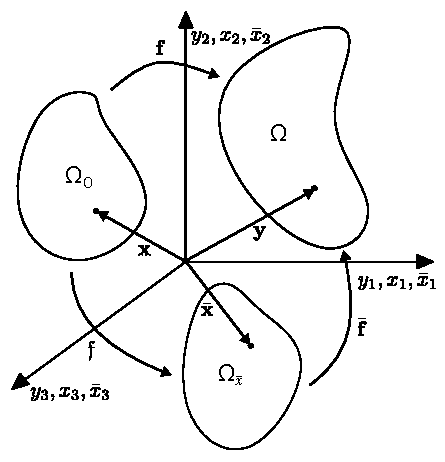
\includegraphics[scale=1.0]{Imagens/Cap2/ALE.pdf}	
	\caption{Domínios utilizados para a descrição Lagrangiana-Euleriana arbitrária}
	\label{fig:Ale}
\end{figure}

Da mesma forma, o domínio de referência, pode ser mapeado a partir do domínio inicial por:

\begin{align}
	\posALE = \mathfrak{f}(\mathbf{x},t).
	\label{eq:PosALE}
\end{align}

A velocidade dos pontos da malha é calcula por:

\begin{align}
	\velocityALE = \left. \frac{\partial \bar{\mathbf{f}}(\posALE,t)}{\partial t} \right|_{\bar{\mathbf{x}}},
\end{align}

\noindent e a velocidade dos pontos materiais no instante $t$ é obtida pela derivada do vetor posição $\pos$ mantendo $\mathbf{x}$ fixo:

\begin{align}
	\velocity = \left. \frac{\partial \mathbf{f}(\mathbf{x},t)}{\partial t} \right|_{\mathbf{x}} = \left. \frac{\partial \pos(\mathbf{x},t)}{\partial t} \right|_{\mathbf{x}}.
\end{align}


As matrizes jacobianas dos mapeamentos considerando a depedência do espaço e do tempo são dadas por:

\begin{equation} \label{eq:ALEJac1}
	\mathbf{F} = \frac{\partial \left(\mathbf{f}(\mathbf{x},t),t\right)}{\partial (\mathbf{x},t)}=
	\begin{bmatrix}
		\frac{\partial {\pos}}{\partial {\mathbf{x}}} & \velocity \\
		\mathbf{0}^T & 1 \\
	\end{bmatrix}
	\text{,}
\end{equation}

\begin{equation} \label{eq:ALEJac2}
	\bar{\mathbf{F}} = \frac{\partial \left(\bar{\mathbf{f}}(\posALE,t),t\right)}{\partial (\posALE,t)}=
	\begin{bmatrix}
		\frac{\partial {\pos}}{\partial {\posALE}} & \velocityALE \\
		\mathbf{0}^T & 1 \\
	\end{bmatrix}
	\text{,}
\end{equation}

e

\begin{equation} \label{eq:ALEJac3}
	\mathfrak{F} = \frac{\partial \left({\mathfrak{f}}(\mathbf{x},t),t\right)}{\partial (\mathbf{x},t)}=
	\begin{bmatrix}
		\frac{\partial {\posALE}}{\partial {\mathbf{x}}} & \mathbf{w} \\
		\mathbf{0}^T & 1 \\
	\end{bmatrix}
	\text{,}
\end{equation}

\noindent sendo $\mathbf{w} = \left. \frac{\partial \posALE}{\partial t} \right|_{\mathbf{x}}$.


Considerando que $\mathbf{f}\left(\mathbf{x},t\right) = \bar{\mathbf{f}} \circ \mathfrak{f}$, pode-se escrever:

\begin{align}
	\frac{\partial(\mathbf{f}(\mathbf{x},t),t)}{\partial(\mathbf{x},t)} = \frac{\partial(\bar{\mathbf{f}}(\posALE,t),t)}{\partial(\posALE,t)} \cdot \frac{\partial(\mathfrak{f}(\mathbf{x},t),t)}{\partial(\mathbf{x},t)},
\end{align}

\noindent que pode ser rescrita como:

\begin{align}
	\begin{bmatrix}
		\frac{\partial {\pos}}{\partial {\mathbf{x}}} & \velocity \\
		\mathbf{0}^T & 1 \\
	\end{bmatrix}
	=
	\begin{bmatrix}
		\frac{\partial {\pos}}{\partial {\posALE}} & \velocityALE \\
		\mathbf{0}^T & 1 \\
	\end{bmatrix}
	\cdot
	\begin{bmatrix}
		\frac{\partial {\posALE}}{\partial {\mathbf{x}}} & \mathbf{w} \\
		\mathbf{0}^T & 1 \\
	\end{bmatrix} .
\end{align}

Dessa forma, pode-se estabelecer uma relação entre a velocidade da malha e a velocidade do ponto material:

\begin{align}
	\velocity = \velocityALE + \frac{\partial{\pos}}{\partial{\posALE}}\cdot \mathbf{w} \label{eq:velRel}
\end{align}

Supondo agora uma grandeza física escalar, denominada de $g(\pos,t)$ na configuração espacial, de $g^{*}(\posALE,t)$ na configuração de referência, e $g^{**}(\mathbf{x},t)$ na configuração material. Pode-se escrever então:

\begin{align}
	g^{**}(\mathbf{x},t) = g(\mathbf{f}(\mathbf{x},t),t), 
\end{align}

\noindent ou:

\begin{align}
	g^{**} = g  \circ \mathbf{f},
\end{align}

\noindent o que permite escrever o seguinte gradiente:

\begin{align}
	\frac{\partial g^{**}(\mathbf{x},t)}{\partial (\mathbf{x},t)} = \frac{\partial g(\pos,t)}{\partial (\pos,t)} \frac{\partial \mathbf{f}(\mathbf{x},t)}{\partial (\mathbf{x},t)},
\end{align}

\noindent que em forma matricial é apresentado como:

\begin{align}
	\begin{bmatrix}
		\frac{\partial {g^{**}}}{\partial {\mathbf{x}}} & \frac{\partial {g^{**}}}{\partial t} \\
	\end{bmatrix}
	=
	\begin{bmatrix}
		\frac{\partial {g}}{\partial \pos} & \frac{\partial {g}}{\partial t} 
	\end{bmatrix}
	\cdot
	\begin{bmatrix}
		\frac{\partial {\pos}}{\partial {\mathbf{x}}} & \velocity \\
		\mathbf{0}^T & 1 \\
	\end{bmatrix} .
\end{align}

Essa expressão nos permite escrever a derivada temporal da variável na configuração material:

\begin{align}
	\frac{\partial g^{**}}{\partial t} = \frac{\partial g}{\partial t} + \frac{\partial g}{\partial \pos} \cdot \velocity, 
\end{align}

\noindent que é justamente a derivada material de g. Para facilitar a visualização pode tirar os sobrescritos $**$, e então:

\begin{align}
	\frac{Dg}{Dt} = \left . \frac{\partial g}{\partial t} \right|_{\mathbf{x}} = \left . \frac{\partial g}{\partial t} \right|_{\pos} + \velocity \cdot \nabla_y g. \label{eq:derMat}
\end{align}

Usando essa mesma metodologia pode-se escrever a transformação de $g^{*}(\bar{\mathbf{x}},t)$ para a referência material da seguinte forma:


\begin{align}
	g^{**} = g^{*}  \circ \mathfrak{f},
\end{align}

\noindent que resulta no seguinte gradiente

\begin{align}
	\begin{bmatrix}
		\frac{\partial {g^{**}}}{\partial {\mathbf{x}}} & \frac{\partial {g^{**}}}{\partial t} \\
	\end{bmatrix}
	=
	\begin{bmatrix}
		\frac{\partial {g^*}}{\partial \posALE} & \frac{\partial {g*}}{\partial t} 
	\end{bmatrix}
	\cdot
	\begin{bmatrix}
		\frac{\partial {\posALE}}{\partial {\mathbf{x}}} & \mathbf{w} \\
		\mathbf{0}^T & 1 \\
	\end{bmatrix},
\end{align}


\noindent com a segunda coluna resultando em:

\begin{align}
	\frac{\partial g^{**}}{\partial t} = \frac{\partial g^*}{\partial t} + \frac{\partial g*}{\partial \posALE} \cdot \mathbf{w}. \label{eq:refMat}
\end{align}

Utilizando-se a expressão apresenta na Eq. \ref{eq:velRel} e substituindo-a em \ref{eq:refMat}, resulta em:

\begin{align}
	\frac{\partial g^{**}}{\partial t} = \frac{\partial g^*}{\partial t} + \frac{\partial g*}{\partial \pos} \cdot \left(\velocity - \velocityALE \right). 
\end{align}

Removendo-se os sobrescritos (**) e (*), chega-se a equação fundamental para os desenvolvimentos utilizando a metodologia ALE:

\begin{align}
	\frac{Dg}{Dt} = \left . \frac{\partial g}{\partial t} \right|_{\mathbf{x}} = \left . \frac{\partial g}{\partial t} \right|_{\posALE} + \left(\velocity - \velocityALE \right) \cdot \nabla_y g. \label{eq:DerMatALE}
\end{align}

Utilizando-se a definição de derivada material da Eq. \ref{eq:derMat} e comparando com a Eq. \ref{eq:Navier-Stokes}, pode-se rescrever a equação da quantidade de movimento da seguinte forma:

\begin{align}
	\density\left(\frac{D\velocity}{Dt} - \sbodyforce \right) - \nabla_y \cdot \stresstensor &= \mathbf{0}. \label{Navier-Stokes-MatDerEuleriana}
\end{align}

Para expressar então a equação da quantidade de movimento em uma descrição Euleriana-Lagrangeana, basta substituir na Eq. \ref{Navier-Stokes-MatDerEuleriana} a definição de derivada material apresentada na Eq. \ref{eq:DerMatALE}, e têm-se finalmente:

\begin{align}
	\density\left(\left. \frac{\partial\velocity}{\partial t} \right|_{\bar{\mathbf{x}}} + \left(\velocity - \velocityALE \right) \cdot \nabla_y  \velocity  - \sbodyforce \right) - \nabla_y \cdot \stresstensor = \mathbf{0}. \label{eq:Navier-StokesALE} 
\end{align}

A equação da continuidade independe da movimentação da malha. Dessa forma a Eq. \ref{eq:conserMassaIncom} se mantém a mesma para as análises usando uma descrição ALE. Assim, reescrevendo o conjunto de equações da DFC apresenta na Eq. \ref{eq:ConjDFC} para um descrição ALE, têm-se:

\begin{equation}
	\left\{
	\begin{array}{l}
		\density\left( \left. \frac{\partial\velocity}{\partial t} \right|_{\posALE}  + \left(\velocity - \velocityALE \right)\cdot\nabla_y\velocity - \sbodyforce \right) - \nabla_y \cdot \stresstensor = \mathbf{0}  \ \textrm{em} \ \domain\\
		\nabla_y \cdot \velocity = 0  \ \textrm{em} \ \domain\\
		\velocity = \velocityD \ \textrm{em} \ \GammaD \\
		\stresstensor \cdot \snormal = \surfaceLoad \ \textrm{em} \ \GammaN,
	\end{array} \label{eq:ConjDFCALE}
	\right.
\end{equation}


\section{Forma fraca e discretização espacial das equações governantes} \label{capitulo:Cap2:FormaFraca}

Tomando-se a forma forte das equações governantes da DFC em descrição ALE, aplica-se o método de resíduos ponderados para se chegar à forma fraca e proceder com a discretização espacial. Os espaços de dimensão finita das funções tentativa que descrevem a velocidade e a pressão são chamados de $\usolution$ e $\psolution$ respectivamente, e definidos como:

\begin{align}
\usolution = \left\{\velocity \left . \right| \velocity \left(\cdot,t\right) \in \left(H^{1}\left(\domain\right)\right)^{n_{sd}}, \velocity = \velocity_D \ \textrm {em} \ \GammaD \right\}
\end{align}

\noindent e

\begin{align}
\psolution = \left\{\press \left . \right| \press \left(\cdot\right) \in L^{2}\left(\domain\right), \int_{\domain}\press \textrm { } d\domain = 0 \textrm { se } \boundary = \GammaN \right\},
\end{align}

\noindent sendo $\left(H^{1}\left(\domain\right)\right)^{n_{sd}}$ o espaço de funções vetoriais com derivadas de quadrado integrável sobre $\domain$ e $L^{2}\left(\domain\right)$ o espaço de funções escalares que são de quadrado integrável sobre $\domain$.

O espaço das funções teste ou funções peso das equações da quantidade de movimento e da continuidade são definidos respectivamente por:

\begin{align}
\uweighting = \left\{\utest \left . \right| \utest \left(\cdot\right) \in \left(H^{1}\left(\domain\right)\right)^{n_{sd}}, \mathbf{w} = 0 \textrm { em} \ \GammaD \right\},
\end{align}


\begin{align}
\pweighting = \psolution.
\end{align}

Aplicando-se o método dos resíduos ponderados sobre as equações Eq. \eqref{eq:Navier-StokesALE} e Eq.\eqref{eq:conserMassaIncom}, integrando-se por partes o termo referente ao tensor de tensões de Cauchy, empregando-se o teorema da divergência e levando-se em consideração a condição de homogeneidade da função $\utest$ sobre o contorno $\boundary_D$, obtém-se a forma fraca. A solução do problema consiste então em encontrar $\velocity \in \usolution$ e $\press \in \psolution$, de tal modo que $\forall$ $\utest \in \uweighting$ e $\ptest \in \pweighting$, as seguintes expressões sejam verdadeiras:


\begin{align}
\int_{\domain} \utest \cdot \density  \left(\left . \frac{\partial\velocity}{\partial t} \right|_{\posALE} + \left(\velocity - \velocityALE \right)\cdot\nabla_y \velocity - \sbodyforce \right) d\domain + \int_{\domain} \straintensor(\utest) : \stresstensor  d\domain - \int_{\GammaN} \utest \cdot \mathbf{h} \  &= 0,  \label{eq:NSWeakForm1} 
\end{align}

\begin{align}
\int_{\domain} \ptest \left(\nabla_y \cdot \velocity\right) d \domain &= 0. \label{eq:CWeakForm1} 
\end{align}


\subsection{Método dos elementos finitos }

Antes de prosseguir com a discretização espacial da forma fraca do conjunto de equações da Mecânica dos Fluidos, é fundamental compreender os princípios básicos do Método dos Elementos Finitos.  A discretização espacial tanto pelo método dos elementos finitos, como pela técnica de análise isogeométrica (Cap. \ref{capitulo:Cap3}), consiste em, dado um problema com domínio $\domain$, dividi-lo em subdomínios $\domain^{e}$, também chamados de elementos ou células, de forma que:

\begin{align}
	\domain \approx \domain^{h} = {\bigcup_{e = 1}^{nel}} \domain^{e},
\end{align}

\noindent onde $\domain^{h}$ é o domínio discretizado por subdomínios, com o índice $h$ se referindo ao tamanho representativo dos elementos, e $nel$ representando o número total de elementos.

Da mesma forma o contorno do domínio também é discretizado da seguinte forma:

\begin{align}
	\boundary \approx \boundary^{h} = {\bigcup_{b = 1}^{neb}} \boundary^{b},
\end{align}

\noindent onde $neb$ representa o número de elementos que formam o contorno.

No Método dos Elementos Finitos, cada subdomínio, denominado elemento, é composto por um conjunto de pontos, chamados nós. As variáveis de interesse do problema, que incluem a geometria na abordagem isoparamétrica, são aproximadas pela combinação linear de um número finito de funções associadas aos nós, chamadas funções de forma, multiplicadas por variáveis chamadas parâmetros nodais. As funções de forma utilizadas no Método dos Elementos Finitos satisfazem, em geral, a propriedade de partição da unidade, ou seja, a soma das funções de forma associadas a todos os nós de um elemento resulta em 1 para qualquer ponto dentro do domínio paramétrico do elemento. A técnica de elementos finitos pode ser estudada nos diversos livros disponíveis sobre o assunto, tais como \citeonline{ZienkiewiczT:2005a,Reddy:2006}.

Nesse trabalho são utilizadas funções de forma quadráticas do tipo polinômios de Lagrange, sendo empregados elementos isoparamétricos triangulares para o caso 2D e tetraédricos para o caso 3D. Na Fig. \ref{fig:elementofinito2d} e Fig. \ref{fig:elementofinito3d}, pode-se observar os elementos finitos 2D e 3D respectivamente bem como os espaços paramétricos adimensionais adotados para definir as funções de forma. 

\begin{figure}[!htb]
	\centering	
	\subfloat[Elemento Finito 2d.\label{fig:elementofinito2d}]{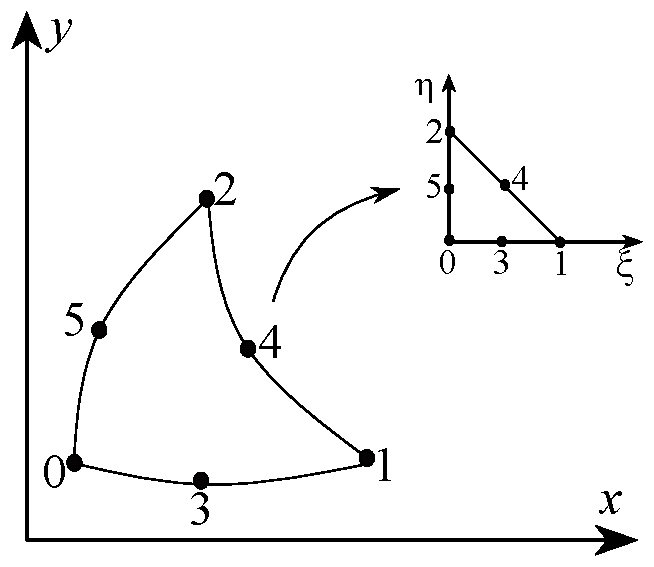
\includegraphics[scale=0.5,trim=0cm 0cm 0cm 0cm, clip=true]{Imagens/Cap2/element2d.pdf}}\\
	\subfloat[Elemento Finito 3d.\label{fig:elementofinito3d}]{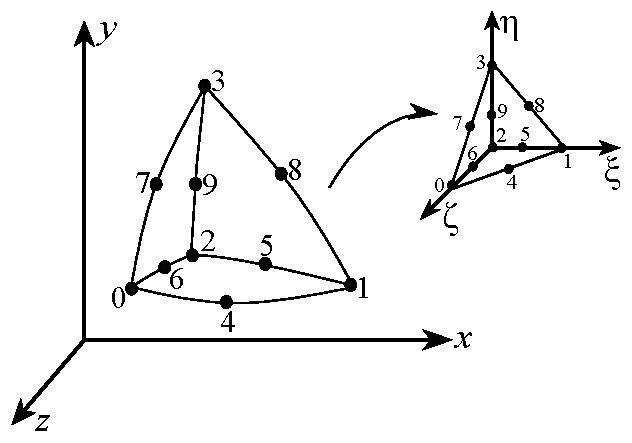
\includegraphics[trim=0 0 0 0,clip,scale=0.65]{Imagens/Cap2/element3d.pdf}}
	\caption{Elementos Finitos: representação espacial e paramétrica}
\end{figure}

Adotar a abordagem isoparamétrica implica que a geometria do problema é descrita também pela combinação entre funções de forma e as coordenadas nodais da malha, conforme equação abaixo:

\begin{align}
	\pos^{h} = \sum_{A = 1}^{N_{nos}} \pos_{A}N_{A}(\pos),
\end{align}

\noindent sendo que para uma geometria tridimensional o vetor $\pos$ possui coordenadas $y_1,y_2$ e $y_3$, as quais representam as posições físicas do domínio; O subíndice "$A$"  representa o índice dos nós da malha, $N_{nos}$ o número total de nós e $N$ as funções de forma da discretização.

A discretização das variáveis de interesse para DFC no contexto do método dos elementos finitos serão apresentados no seguinte capítulo (Cap. \ref{capitulo:Cap2:DiscEspacial}).


\subsection{Discretização Espacial} \label{capitulo:Cap2:DiscEspacial}

Os espaços de função tentativa para velocidade e pressão, bem como as funções teste, no contexto dos método dos elementos finitos, são dados pela combinação linear de parâmetros nodais com funções de forma definidas sobre cada subdomínio, atendendo à partição da unidade, de forma que o problema da dinâmica dos fluidos fica definido como: encontrar $\velocityh \in \usolutionh$ e $\pressh \in \psolutionh$, de tal modo que $\forall$ $\utesth \in \uweightingh$ e $\ptesth \in \pweightingh$ a seguinte expressão seja verdadeira:

\begin{align}
	\begin{split}
		&\int_{\domain} \utesth \cdot \density \left(\left. \frac{\partial\velocityh}{\partial t} \right|_{\posALE} + \left(\velocityh - \velocityALEh \right)\cdot\nabla_y \velocityh - \sbodyforce^{h}\right) d\domain + \int_{\domain} \straintensor(\utesth) : \stresstensor\left(\velocityh,\pressh \right)  d\domain\\ & - \int_{\GammaN} \utesth \cdot \mathbf{h}^{h} + \int_{\domain} \ptesth \left(\nabla_y \cdot \velocityh\right) d \domain = 0,  \label{eq:NSWeakForm2} 
	\end{split}
\end{align}

\noindent onde:

\begin{align}
\velocity^{h}(\pos,t) = \sum_{A = 1}^{N_{nos}} \velocity_{A}(t)N_{A}(\pos), \label{eq:dis_vel}
\end{align}

\begin{align}
\press^{h}(\pos,t)  = \sum_{A = 1}^{N_{nos}} \press_{A}(t)N_{A}(\pos),
\end{align}

\begin{align}
\utest^{h}(\pos)  = \sum_{A = 1}^{N_{nos}} \utest_{A}N_{A}(\pos), \label{eq:utest}
\end{align}

\begin{align}
\ptest^{h}(\pos)  = \sum_{A = 1}^{N_{nos}} \ptest_{A}N_{A}(\pos), \label{eq:ptest} 
\end{align}

\noindent sendo as variáveis $\utest_{A}$ e $\ptest_{A}$ arbitrárias nas aproximações.

No entanto, as formulações obtidas pelo método de Galerkin são conhecidas por apresentarem oscilações espúrias em escoamentos dominados pela convecção. Uma das formas de se lidar com esse problema é a utilização de métodos estabilizados, como \textit{Streamline-Upwind/Petrov-Galerkin} (SUPG) \cite{BrooksH:1982, HughesT:1984}, aplicado nesse trabalho. Essa metodologia consiste em adicionar à equação da quantidade de movimento, o seu resíduo ponderado por $\SUPG \left(\left(\velocityh - \velocityALEh \right) \cdot \nabla_y\utesth\right)$, onde $\SUPG$ é um parâmetro de estabilização. Do ponto de vista numérico a aplicação de  sobre o termo convectivo da equação da quantidade de movimento dá origem a um termo difusivo adicional, cuja viscosidade tem magnitude $\SUPG$, e é responsável por garantir a estabilidade numérica em problemas com convecção dominante.

Para os problemas de escoamentos incompressíveis aqui analisados, deve-se levar em conta que os campos de velocidade e pressão não podem ser aproximados arbitrariamente, podendo levar à ocorrência de oscilações espúrias no campo de pressão. Para evitar isso, podem ser escolhidos elementos Taylor-Hood que obedeçam, à condição de \textit{Ladyzhenskaya-Babuška-Brezzi} (LBB) \cite{BrezziF:1991,ZienkiewiczTN:2005,StrangF:2008}, ou pode-se recorrer a um método estabilizado. 

Neste trabalho, para estabilização da pressão, emprega-se a técnica \textit{Pressure Stabilization Petrov Galerkin} (PSPG)   \cite{HughesFB:1986,TezduyarMRS:1992a}. Essa técnica consiste em adicionar à equação da continuidade, o resíduo da equação da quantidade de movimento ponderada pela função $\PSPG \left(\frac{\nabla_y \ptesth}{\density}\right)$, onde $\PSPG$ é um parâmetro de estabilização. Essa estabilização cria termos dependentes da pressão na equação da continuidade, responsáveis pela flexibilização do campo de pressão e por contornar a condição LBB.

Por fim, para prover maior estabilização em problemas com formação de vórtices, adiciona-se à equação da quantidade de movimento o resíduo da equação da continuidade ponderado por $ \LSIC \density \left(\nabla_y \cdot \utesth\right)$ \cite{TezduyarO:2000}, sendo $\LSIC$ um parâmetro de estabilização. A estabilização  $\LSIC$ dá origem a um termo do tipo mínimos quadrados, e que também introduz na formulação uma difusão artificial.

Nota-se que a consistência da formulação estabilizada é garantida, uma vez que são adicionados às equações seus resíduos ponderados. Os parâmetros de estabilização $\SUPG$, $\PSPG$ e $\LSIC$ têm função de proporcionar uma solução estável e otimizar a convergência durante o refinamento de malha. A obtenção dos parâmetros estabilizadores será discutida na Subseção \ref{subsec:taus}. 

Por fim, o problema da dinâmica dos fluidos passa a ser a determinação de $\velocityh \in \usolutionh$ e $\pressh \in \psolutionh$, de tal modo que $\forall$ $\utesth \in \uweightingh$ e $\ptesth \in \pweightingh$ as seguintes expressões sejam verdadeiras:

\begin{align}
\begin{split}
&\int_{\domain} \utesth \cdot \density\left(\left. \frac{\partial\velocityh}{\partial t}\right|_{\posALE}+ \left(\velocityh - \velocityALEh \right) \cdot \nabla_y \velocityh - \sbodyforce^h\right) d\domain +\int_{\domain} \straintensor \left(\utesth\right) : \stresstensor \left(\velocityh,\pressh\right)\ d\domain\\ &
- \int_{\boundary_N}\utesth \cdot \straction^h\ d\GammaN \\ 
&+ \sum_{e=1}^{\nel} \int_{\domainE} \SUPG \left(\left(\velocityh - \velocityALEh \right) \cdot \nabla_y \utesth\right) \cdot \resMom\left(\velocityh,\pressh \right)\  d\domain\\
&+ \sum_{e=1}^{\nel} \int_{\domainE} \density \LSIC \nabla_y \cdot \utesth \resPre\left(\velocityh\right)\  d\domain = 0,
\label{eq:FinalSystem}
\end{split}
\end{align}

\noindent e

\begin{align}
	\begin{split}
	&\int_{\domain}\ptesth \nabla_y \cdot \velocityh \ d\domain \\ 
	&+ \sum_{e=1}^{\nel} \int_{\domainE} \PSPG \left(\frac{\nabla_y \ptesth}{\density}\right) \cdot \resMom\left(\velocityh,\pressh\right) \  d\domain = 0,
	\label{eq:RC}
	\end{split}
	\end{align}

\noindent onde $\resMom$ e $\resPre$ são os resíduos da equação da quantidade de movimento e da equação da continuidade, respectivamente, dados por:

\begin{align}
\resMom\left(\velocityh,\pressh\right)&=\density\left(\left. \frac{\partial\velocityh}{\partial t}\right|_{\posALE}+\left(\velocityh - \velocityALEh \right)\cdot \nabla_y \velocityh - \sbodyforce^h\right) - \nabla_y \cdot \stresstensor\left(\velocityh,\pressh\right),
\end{align}

\noindent

\begin{align}
\resPre\left(\velocityh\right)&=\nabla_y \cdot \velocityh.
\end{align}

Visto que existem funções teste separadas para a velocidade e pressão, pode-se definir dois vetores residuais correspondentes a equação da quantidade de movimento ($\NNSM$) e a equação da continuidade ($\NNSC$). Considerando a arbitrariedade de $\utest_{A}$ e $\ptest_{A}$, têm-se:

\begin{align}
\NNSM  = [\left(\NNSM\right)_{A,i}],
\end{align}

\begin{align}
	\NNSC =  [\left(\NNSC\right)_{A}],
\end{align}
	
\noindent com:

\begin{align}
	\begin{split}
	\left(\NNSM\right)_{A,i} =&\int_{\domain} N_{A}\mathbf{e_i} \cdot \density\left(\left. \frac{\partial\velocityh}{\partial t}\right|_{\posALE}+\left(\velocityh - \velocityALEh \right)\cdot \nabla_y \velocityh - \sbodyforce^h\right) d\domain +\int_{\domain} \straintensor \left(N_{A}\mathbf{e_i}\right) : \stresstensor \left(\velocityh,\pressh\right)\ d\domain\\ &
	- \int_{\boundary_N}N_{A}\mathbf{e_i} \cdot \straction^h\ d\GammaN\\ 
	&+ \sum_{e=1}^{\nel} \int_{\domainE} \SUPG \left(\left(\velocityh - \velocityALEh \right) \cdot \nabla_y N_{A}\mathbf{e_i}\right) \cdot \resMom\left(\velocityh,\pressh \right)\  d\domain\\
	&+ \sum_{e=1}^{\nel} \int_{\domainE} \density \LSIC \left(\nabla_y \cdot N_{A}\mathbf{e_i}\right) \resPre\left(\velocityh\right)\  d\domain  ,
	\end{split}
\end{align}

\noindent e:

\begin{align}
	\begin{split}
	\left(\NNSC\right)_{A} = &\int_{\domain} N_A \nabla_y \cdot \velocityh \ d\domain \\ 
	&+ \sum_{e=1}^{\nel} \int_{\domainE} \PSPG \left(\frac{\nabla_y N_A}{\density}\right) \cdot \resMom\left(\velocityh,\pressh\right) \  d\domain,
	\end{split}
\end{align}

\noindent com $i=1,2$ para problemas 2D e $i=1,3$ para problemas 3D.
		
Considerando $\Acceleration$, $\Velocity$ e $\Press$ os vetores nodais dos graus de liberdade respectivos a velocidade, aceleração e pressão, pode-se escrever a forma semidiscreta do problema da DFC como: Encontrar $\Acceleration$, $\Velocity$ e $\Press$ de maneira que

\begin{align}
\NNSM(\Acceleration,\Velocity,\Press) = \mathbf{0},\label{eq:momentum_residual}
\end{align}

\noindent e

\begin{align}
\NNSC(\Acceleration,\Velocity,\Press) = \mathbf{0}. \label{eq:continuity_residual}
\end{align}




\subsection{Parâmetros de estabilização}\label{subsec:taus}

Considerando que nesse trabalho dois tipos de aproximações espaciais são utilizadas, uma baseada no FEM e outra baseada em IGA, adotam-se os parâmetros propostos por \citeonline{TakizawaTO:2018} e \citeonline{OtoguroTT:2020}, que são adequados para ambas aproximações. 

Para essa opção é necessário definir-se o tensor métrico do elemento no espaço. Para isso, inicia-se com a definição da matriz Jacobiana $\matrixQ$, dada por:

\begin{align}
	\matrixQ&=\left(\frac{\partial\pos}{\partial\coordAdimen}\right),
\end{align}

\noindent com $\coordAdimen$ representando as coordenadas do espaço paramétrico, com componentes $\xi_1, \xi_2$ e $\xi_3$.

Para que a ordem polinomial seja levada em consideração na determinação dos parâmetros de estabilização, aplica-se uma mudança de escala na matriz $\matrixQ$, através da matriz $\matrixD$, conforme a seguinte expressão:

\begin{align}
	\matrixQhat&=\matrixQ\matrixD^{-1}.
\end{align}

Para elementos finitos com funções de forma polinomiais de Lagrange de ordem $p_{i}$, na direções $\xi_i$ do espaço paramétrico , com $-1\leq\xi_i\leq1$, a  matriz $\matrixD$ é definida como:


\textcolor{red}{e se a variação for de 0,1 ? tem alguma diferença}

\begin{align}
	\matrixD&=\begin{bmatrix}
		p_{\xi_1} & 0 & 0\\
		0 & p_{\xi_2} & 0 \\
		0 & 0 & p_{\xi_3}
	\end{bmatrix}.
\end{align}

A definição da matriz $\matrixD$ para elementos isogeométricos será descrita na Subseção \ref{subsec:taus2}.

O comprimento direcional do elemento é definido como:

\begin{align}
	\RQD &=2\left(\rRGN\rRGN : \matrixG \right)^{-\frac{1}{2}},
\end{align}

\noindent sendo $\rRGN$ o vetor unitário na direção do gradiente da intensidade da velocidade e $\matrixG$ o tensor métrico do elemento, os quais são representados respectivamente como:

\begin{align}
	\rRGN&=\frac{\nabla_y \lVert\velocityh - \velocityALEh\rVert}{\lVert \nabla_y \lVert\velocityh - \velocityALEh\rVert\rVert} \label{eq:erRGN}
\end{align}

\noindent e

\begin{align}
	\matrixG &= \matrixQhat^{-T} \cdot \matrixQhat^{-1}. 
\end{align}

O comprimento do elemento é limitado pelos mínimos e máximos valores representados abaixo:

\begin{align}
	h_{min} \equiv 2\min_{r}\left((\rRGN\rRGN:\matrixG)^{-\frac{1}{2}} \right), \\
	h_{max} \equiv 2\max_{r}\left((\rRGN\rRGN:\matrixG)^{-\frac{1}{2}} \right),
\end{align}

\noindent que podem ser reescritos como:

\begin{align}
	h_{min} = 2\left(\lambda_{max}\matrixG\right)^{-\frac{1}{2}}, \\
	h_{max} = 2\left(\lambda_{min}\matrixG\right)^{-\frac{1}{2}},
\end{align}

\noindent onde $\lambda_{max}$ e $\lambda_{min}$ representam os máximos e mínimos autovalores da matriz $\matrixG$. 

Os parâmetros de estabilização são dados por:

\begin{align}
	\SUPG = \PSPG =\left(\frac{1}{\SUGNi^2} + \frac{1}{\SUGNii^2} + \frac{1}{\SUGNiii^2} \right)^{-\frac{1}{2}},
\end{align}

\begin{align}
	\LSIC = \frac{\RQD^2}{\SUPG},
\end{align}

\noindent onde:

\begin{align}
	\SUGNi^{-2} = \left(\velocityh - \velocityALEh \right) \left(\velocityh - \velocityALEh \right) : \matrixG ,
\end{align}

\begin{align}
	\SUGNii&=\frac{\Delta t}{2},
\end{align}

\noindent e

\begin{align}
	\SUGNiii^{-1} = \kviscosity \left(\rRGN_{reg}\rRGN_{reg} : \matrixG + \left(1 - \rRGN_{reg}^2)4h_{min}^{-2} \right)\right) ,
\end{align}

\noindent sendo $\rRGN_{reg}$ definido como:

\begin{align}
	\rRGN_{reg} =\frac{\nabla_y \lVert\velocityh - \velocityALEh\rVert}{\lVert \nabla \lVert\velocityh - \velocityALEh\rVert\rVert + \varepsilon\left(\lVert \nabla_y \lVert\velocityh - \velocityALEh\rVert\rVert\right)_0},
\end{align}

\noindent com $\varepsilon$ uma constante pequena e $\left(\lVert \nabla_y \lVert\velocityh- \velocityALEh\rVert\rVert\right)_0$ um valor de referência. Os termos $\SUGNi$, $\SUGNii$ e $\SUGNiii$ são parâmetros correspondentes aos termos convectivos, inerciais e viscosos, respectivamente.

\section{Integração Temporal}\label{sec:IntegTemp}

Para a integração temporal das equações governantes, utiliza-se o método $\alpha$-generalizado. Esse método foi proposto inicialmente por \citeonline{ChungH:1993} no contexto da mecânica das estruturas, e foi estendido para o contexto da dinâmica dos fluidos computacional por \citeonline{JansenWH:2000}.

Considerando que o tempo da análise do problema é definido por um intervalo de $[0,T]$, o qual é particionado em subintervalos $\Delta t_{n} = t_{n+1} - t_{n}$, com $t_{n}$ e $t_{n+1}$ os instantes anterior e atual, respectivamente. A solução do problema consiste em: conhecida a solução nos graus de liberdade nodais ($\Acceleration$, $\Velocity$ e $\Press$) no passo de tempo $n$, encontrar a solução no passo de tempo $n+1$ de forma que:

\begin{align}
\NNSM(\Acceleration_{n+\alpham},\Velocity_{n+\alphaf},\Press_{n+1}) = \mathbf{0}, \label{eq:momentum_residual_alpha}\\
\NNSC(\Acceleration_{n+\alpham},\Velocity_{n+\alphaf},\Press_{n+1}) = \mathbf{0}, \label{eq:continuity_residual_alpha}
\end{align}

\noindent com:

\begin{gather}
\Acceleration_{n+\alpham} = \Acceleration_n + \alpham \left( \Acceleration_{n+1} - \Acceleration_n \right), \label{eq:approx_acceleration}\\
\Velocity_{n+\alphaf} = \Velocity_n + \alphaf \left( \Velocity_{n+1} - \Velocity_n \right), \label{eq:approx_velocity}
\end{gather}

\noindent sendo $\Acceleration_{n+\alpham}$ e $\Velocity_{n+\alphaf}$ valores intermediários entre $t_{n}$ e $t_{n+1}$ do vetor aceleração e velocidade. A relação entre os valores nodais de aceleração e velocidade são calculados de acordo com fórmula discreta de Newmark (ver, por exemplo, \cite{Hughes:1976}):

\begin{gather}
\Velocity_{n+1} = \Velocity_n + \timeStep\left(\left(1-\gamma\right)\Acceleration_n + \gamma\Acceleration_{n+1} \right). \label{eq:newmark}
\end{gather}

Os parâmetros que definem o instante intermediário, no qual as variáveis serão calculadas, são determinados de forma a proporcionarem estabilidade e precisão ao método. Seguindo a metodologia proposta por \citeonline{JansenWH:2000}, uma precisão de segunda ordem é obtida, para casos lineares, desde que: 

\begin{gather}
\gamma = 1/2 + \alpham - \alphaf,\label{eq:gamma}
\end{gather}

\noindent enquanto que a estabilidade do problema é incondicional com:

\begin{gather}
\alpham \ge \alphaf \ge 1/2.
\end{gather}

Para proporcionar a precisão de segunda-ordem de convergência e estabilidade da solução, pode-se calcular o parâmetro $\gamma$ de acordo com Eq. \ref {eq:gamma} e $\alpham$, $\alphaf$, através de \cite{Hughes:2000}:


\begin{gather}
\alpham = \frac{1}{2}\left(\frac{3 - \specRadius}{1+\specRadius}\right)\label{eq:alpha_m_fluid}\\
\end{gather}

\noindent e

\begin{gather}
\alphaf = \frac{1}{1+\specRadius}\label{eq:alpha_f_fluid}.
\end{gather}

O parâmetro $\specRadius$ é conhecido como raio espectral da matriz de amplificação quando $\Delta t_{n} \rightarrow \infty$. Esse parâmetro controla a dissipação numérica em altas frequências realizada pelo processo de integração e está contido no intervalo de $[0,1]$. Para $\specRadius = 0$ a dissipação é máxima e para $\specRadius = 1$ não há introdução de difusão numérica ao método.

Para a solução do sistema de equações não lineares compostas por Eq. \eqref{eq:momentum_residual_alpha} e Eq. \eqref{eq:continuity_residual_alpha} utiliza-se o método de Newton-Raphson. O método pode ser separado em duas etapas, uma etapa preditiva e outra iterativa corretiva \cite{BazilevsTT:2013}.

Na etapa preditiva, conhecida a solução em um passo de tempo $n$, prediz-se a solução em $n+1$ com as seguintes equações:

\begin{align}
\Acceleration_{n+1}^{0} = \frac{\gamma-1}{\gamma}\Acceleration_{n} \label{eq:Pred1},
\end{align}

\begin{align}
\Velocity_{n+1}^{0} = \Velocity_{n}, \label{eq:Pred2}
\end{align}

\begin{align}
\Press_{n+1}^{0} = \Press_{n},\label{eq:Pred3}
\end{align}

\noindent onde o índice $0$ representa a iteração de número zero. 

Na etapa iterativa corretiva, itera-se sobre a Eq. \eqref{eq:momentum_residual_alpha} e Eq. \eqref{eq:continuity_residual_alpha} até que elas sejam satisfeitas, considerando uma tolerância prescrita, ou até que se alcance uma quantidade máxima de iterações pré-estabelecida. Essa etapa é composta por três fases. A fase 1 consiste em determinar os valores no instante intermediário para as variáveis nodais na iteração $i$:

\begin{align}
\Acceleration_{n+\alpham}^{i} = \Acceleration_n + \alpham \left( \Acceleration_{n+1}^{i} - \Acceleration_n \right), \label{eq:approx_accelerationI}\\
\Velocity_{n+\alphaf}^{i} = \Velocity_n + \alphaf \left( \Velocity_{n+1}^{i} - \Velocity_n \right), \label{eq:approx_velocityI}\\
\Press_{n+1}^{i} = \Press_{n+1}^{i} \label{eq:approx_pressI}.
\end{align}

Na fase 2, com os valores intermediários das variáveis nodais resolve-se o sistema linear resultante da linearização das equações Eq. \eqref{eq:momentum_residual_alpha} e Eq. \eqref{eq:continuity_residual_alpha} com respeito às variáveis de interesse $\Press_{n+1}$ e $\Acceleration_{n+1}$:

\begin{align}
\left .\frac{\partial\NNSM}{\partial\Acceleration_{n+1}}\right|_{i} \Delta \Acceleration_{n+1}^{i} + \left .\frac{\partial\NNSM}{\partial\Press_{n+1}}\right|_{i} \Delta \Press_{n+1}^{i} = -\NNSM^{i}, \label{eq:NR1} \\
\left .\frac{\partial\NNSC}{\partial\Acceleration_{n+1}}\right|_{i} \Delta \Acceleration_{n+1}^{i} + \left .\frac{\partial\NNSC}{\partial\Press_{n+1}}\right|_{i} \Delta \Press_{n+1}^{i} = -\NNSC^{i}.\label{eq:NR2}
\end{align}

Por fim, na fase 3 atualiza-se a solução através das seguintes relações:

\begin{align}
\Acceleration_{n+1}^{i+1} = \Acceleration_{n+1}^{i} + \Delta\Acceleration_{n+1}^{i},\label{update1} \\ 
\Velocity_{n+1}^{i+1} = \Velocity_{n+1}^{i} + \gamma \Delta t \Delta\Velocity_{n+1}^{i},\label{update2}\\
\Press_{n+1}^{i+1} = \Press_{n+1}^{i} + \Delta\Press_{n+1}^{i}.\label{update3}
\end{align}

Na utilização do método $\alpha$-generalizado as integrais das equações Eq. \eqref{eq:momentum_residual_alpha} e Eq. \eqref{eq:continuity_residual_alpha} são avaliadas no instante $t = t_{n+\alpha_{f}}$, de forma que:

\begin{align}
\int_{\domain_{t}} \left(.\right) d\domain = \int_{\domain_{t_{n+\alpha_{f}}}} \left(.\right) d\domain
\end{align}

\begin{align}
\domainALEN = \left\{\posh \  |\  \posh(\posALEh,t_{(n+\alphaf)}) = \alphaf \posh(\posALEh,t_{n+1}) + (1-\alphaf) \posh(\posALEh,t_n)  \right\}.
\end{align}





\subsection{Implementação Computacional} \label{subsection:DFCComputationalCode}


O Algoritmo que descreve a implementação computacional tanto de problemas utilizando o método dos elementos finitos, quanto para problemas utilizando a análise Isogeométrica, é apresentado no Alg. \ref{alg:fluid_temporalIntegration}.

\begin{algorithm}
	\caption{Algoritmo para problemas de dinâmica dos fluidos computacional}
	\label{alg:fluid_temporalIntegration}
	\begin{algorithmic}[1]
		\For {o passo de tempo $0$ até \timeInterval} 
		\State $i=0$;
		\State Predição da solução: aplicação das Eq. \eqref{eq:Pred1}, Eq. \eqref{eq:Pred2} e Eq. \eqref{eq:Pred3};
		\While{($\epsilon$ < tolerância)}
		\State $i$++;
		\State Interpolação das variáveis do problema: aplicação da Eq. \eqref{eq:approx_accelerationI}, Eq. \eqref {eq:approx_velocityI} e Eq. \eqref{eq:approx_pressI};
		\State Cálculo do incremento nas variáveis do problema: $\Acceleration_{n+1}$ e $\Press_{n+1}$ de acordo com as Eq. \eqref{eq:NR1} e Eq. \eqref{eq:NR2};
		\State Atualização da solução: calculadas de acordo com Eq. \eqref{update1}, Eq. \eqref{update2} e Eq. \eqref{update3}.
		\State Cálculo do erro:
		\begin{align}
		\epsilon =\left\| \NNSM^i \right\|_{L^2}
		\end{align}
		\EndWhile
		\EndFor
	\end{algorithmic}
\end{algorithm}



\section{Verificação e Aplicações}

Para a verificação dos códigos baseados no método dos elementos finitos, adotam-se 2 exemplos muito populares nas bibliografias: Escoamento sobre um cilindro 2D e o problema da cavidade quadrada 3D, os quais são apresentados na subseções sequentes.

\subsection{Escoamento sobre um cilindro - 2D} \label{subsection:escoamentocil2d}

O estudo do problema de um escoamento sobre um cilindro 2D teve como principal intuito a análise dos coeficientes aerodinâmicos medidos ao longo do tempo e verificar consequentemente se o modelo é capaz de reproduzir os fenômenos relacionados à formação e desprendimento de vórtices característicos desse problema. Para isso, diferentes números de Reynolds ($\Reynolds$) foram estudados, $\Reynolds$ = 40, 100 e 1000, os quais são calculados de acordo com a seguinte equação:

\begin{align}
	\Reynolds = \frac{\rho L \lVert\velocinfty\lVert}{\viscosity} = \frac{L \lVert \velocinfty \lVert}{\kviscosity}, \label{eq:Reynolds}
\end{align}

\noindent com $L$ a dimensão característica do problema, sendo nesse caso o diâmetro do cilindro, e $\kviscosity$ a viscosidade cinemática do fluido. 

\begin{figure}[!htb]
	\centering
	\subfloat[Geometria e condições de contorno.\label{fig:cilindro2d_geometria}]{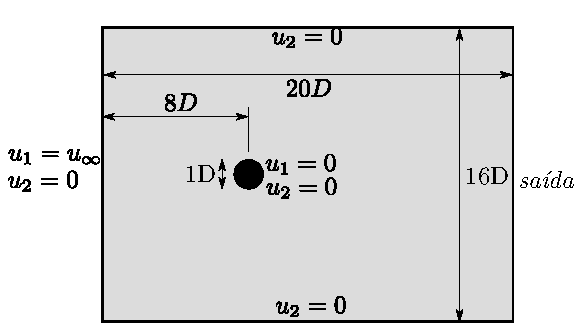
\includegraphics[scale=1.0,trim=0cm 0cm 0cm 0cm, clip=true]{Imagens/Cap2/cilindro2d.pdf}}\\
	\subfloat[Discretização espacial.\label{fig:cilindro2d_malha}]{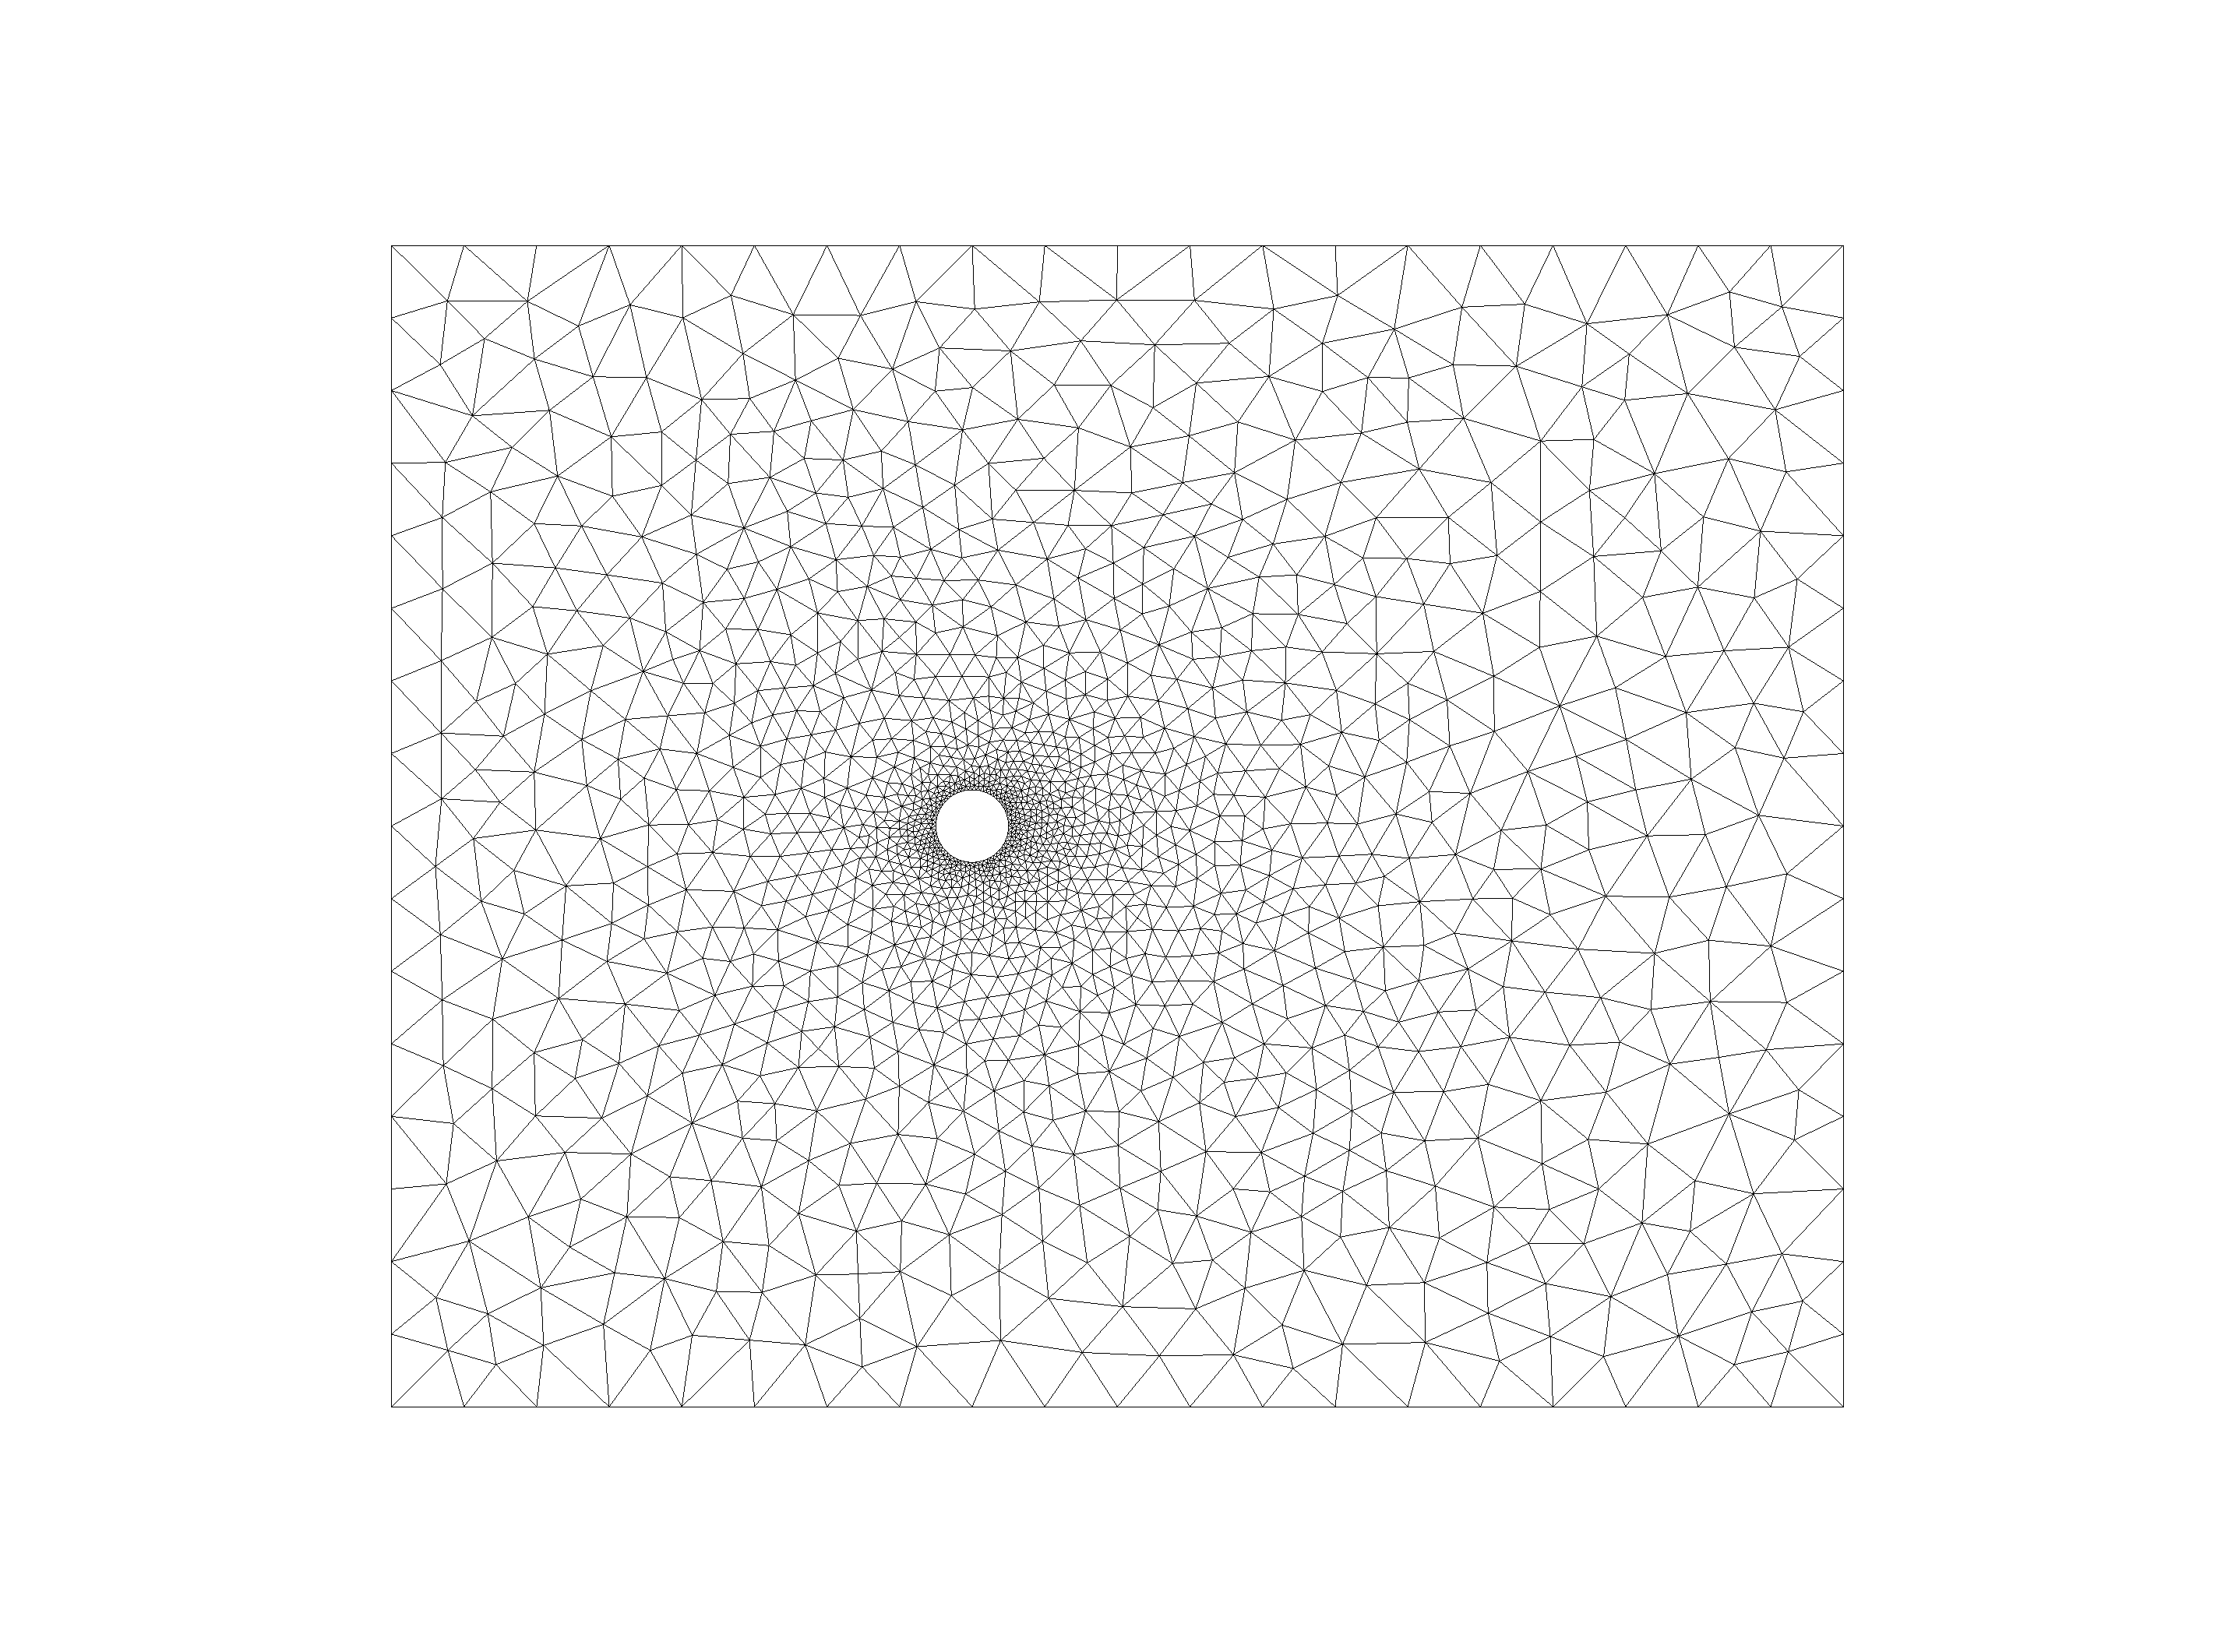
\includegraphics[trim=170 120 170 130,clip,scale=0.2]{Imagens/Cap2/MeshCylinder2D.eps}}
	\caption{Cilindro 2D: Geometria, condições de contorno e malha de elementos finitos.}
\end{figure}


A geometria e condições de contorno são apresentadas na Fig. \ref{fig:cilindro2d_geometria}. Como pode-se observar trata-se de um domínio retangular, parametrizado em função do diâmetro do cilindro, com um perfil constante de velocidade na entrada e condição de parede lisa nas paredes superior e inferior. No contorno denominado como \textit{saída}, não se conhece o comportamento do escoamento, desta forma, determina-se sua posição no domínio computacional a uma distância grande o suficiente de maneira a não interferir no comportamento do escoamento. 

Na Fig. \ref{fig:cilindro2d_malha} pode-se observar a malha não-estruturada de elementos finitos utilizada para esse problema, composta por 3122 elementos triangulares quadráticos e 6376 nós. O problema foi simulado para um velocidade de entrada $u_{\infty} = 1,0$, $\rho = 1,0$, $\timeStep = 0,05$, e $\specRadius = 0,5$. 

Para o cálculo dos coeficientes aerodinâmicos é necessário definir-se primeiramente as forças de arrasto - horizontal ($F_D$) e de sustentação - vertical ($F_L$), que são induzidas por tensões desviadores e hidrostáticas e são calculadas pelas seguintes equações:

\begin{align}
F_D = \int_{\boundary_{c}} \stresstensor_{1j}n_{j} d\boundary_{c},
\end{align}

\begin{align}
F_L = \int_{\boundary_{c}} \stresstensor_{2j}n_{j} d\boundary_{c},
\end{align}

\noindent nas quais o símbolo $\boundary_{c}$ representa o contorno do cilindro e $_jn$ é o vetor normal à essa superfície na direção $j$, com $j=1,2$. Os coeficientes de arrasto e sustentação são definidos respectivamente por:

\begin{align}
	C_D = \frac{F_D}{0,5\rho \lVert \velocity_{\infty} \lVert^{2} L},
\end{align}

\begin{align}
	C_L = \frac{F_L}{0,5\rho \lVert \velocity_{\infty} \lVert^{2} L},
\end{align}.

Devido ao fenômeno de desprendimento de vórtices que ocorre a partir de determinado número de Reynolds do escoamento, é usual determinar-se a frequência deste fenômeno através do número adimensional de Strouhal ($\Strouhal$), dado por:

\begin{align}
	\Strouhal = \frac{f_{V}L}{\lVert \velocity_{\infty} \lVert},
\end{align}.

\noindent com $f_{V}$ sendo a frequência de desprendimento dos vórtices.

Como pode-se observar na Fig. \ref{fig:cilindro_coeficientes} para $\Reynolds = 40$, os coeficientes de arrasto e de sustentação, após o escoamento entrar em fase estacionária, se mantém constantes ao longo de todo o tempo de análise. Isso ocorre, visto que para Reynolds entre 5 à 50, aproximadamente, formam-se dois vórtices simétricos e estacionários na região logo após o cilindro. Posteriormente, o par de vórtices se quebra e passa existir a chamada esteira de Von Karmán, que ocorre devido à formação de vórtices de maneira alternada entre as regiões superior e inferior do cilindro, o que pode ser notado também na Fig. \ref{fig:cilindro_coeficientes}  para $Re = 100$ e $Re=1000$. Os valores do coeficiente de Strouhal, para $Re = 100$ e $Re=1000$, foram de 0,1716 e 0,2454 respectivamente. Os valores obtidos para os coeficientes aerodinâmicos foram os esperados para o problema em questão (ver, por exemplo, \citeonline{Tonon:2016,Henderson:1997}).

\begin{figure}[!htb]
	\centering
	\subfloat[\label{fig:cilindro_Cd}Coeficiente de arrasto $ C_D$.]{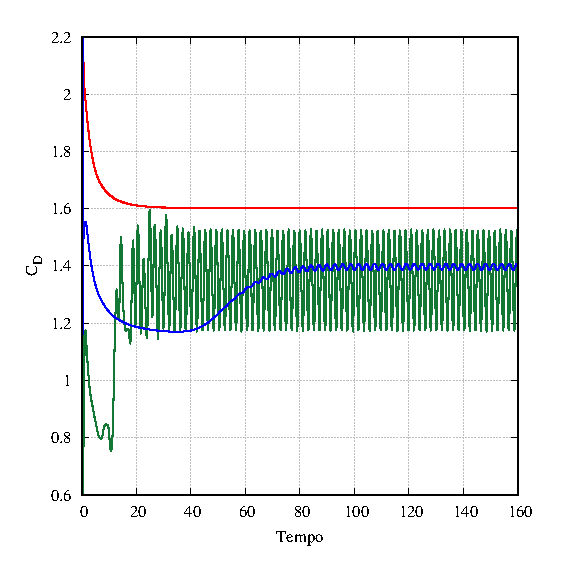
\includegraphics[scale=1,trim=0cm 0cm 0cm 0cm, clip=true]{Imagens/Cap2/DragRe.eps}}\\ 
	\subfloat[\label{fig:cilindro_Cl}Coeficiente de sustentação $C_L$.]{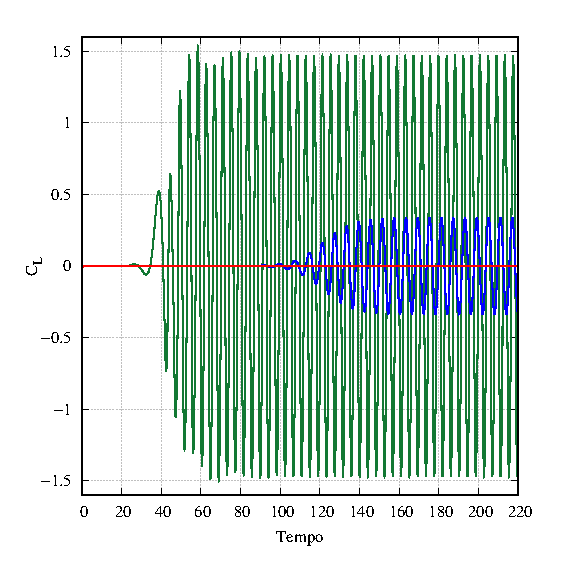
\includegraphics[scale=1,trim=0cm 0cm 0cm 0cm, clip=true]{Imagens/Cap2/LiftRe.eps}}\\ 
	{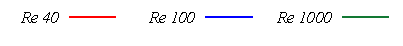
\includegraphics[scale=1.3]{Imagens/Cap2/Legenda.pdf}}
	\caption{Cilindro 2D: Coeficientes aerodinâmicos. }
	\label{fig:cilindro_coeficientes}
\end{figure}

Nas Fig. \ref{fig:cilindro_2d_pressao} e Fig. \ref{fig:cilindro_2d_velocidade} podem ser observados os campos de pressão e velocidade em um tempo $t=11,5$ da análise para $Re = 100$. Pode-se notar nessas imagens, a formação e os desprendimentos de vórtices na esteira de Von Karmán, característico do escoamento para o número de Reynolds simulado.

\begin{figure}[!htb]
	\centering
	\subfloat[\label{fig:cilindro_2d_pressao}Campo de pressão]{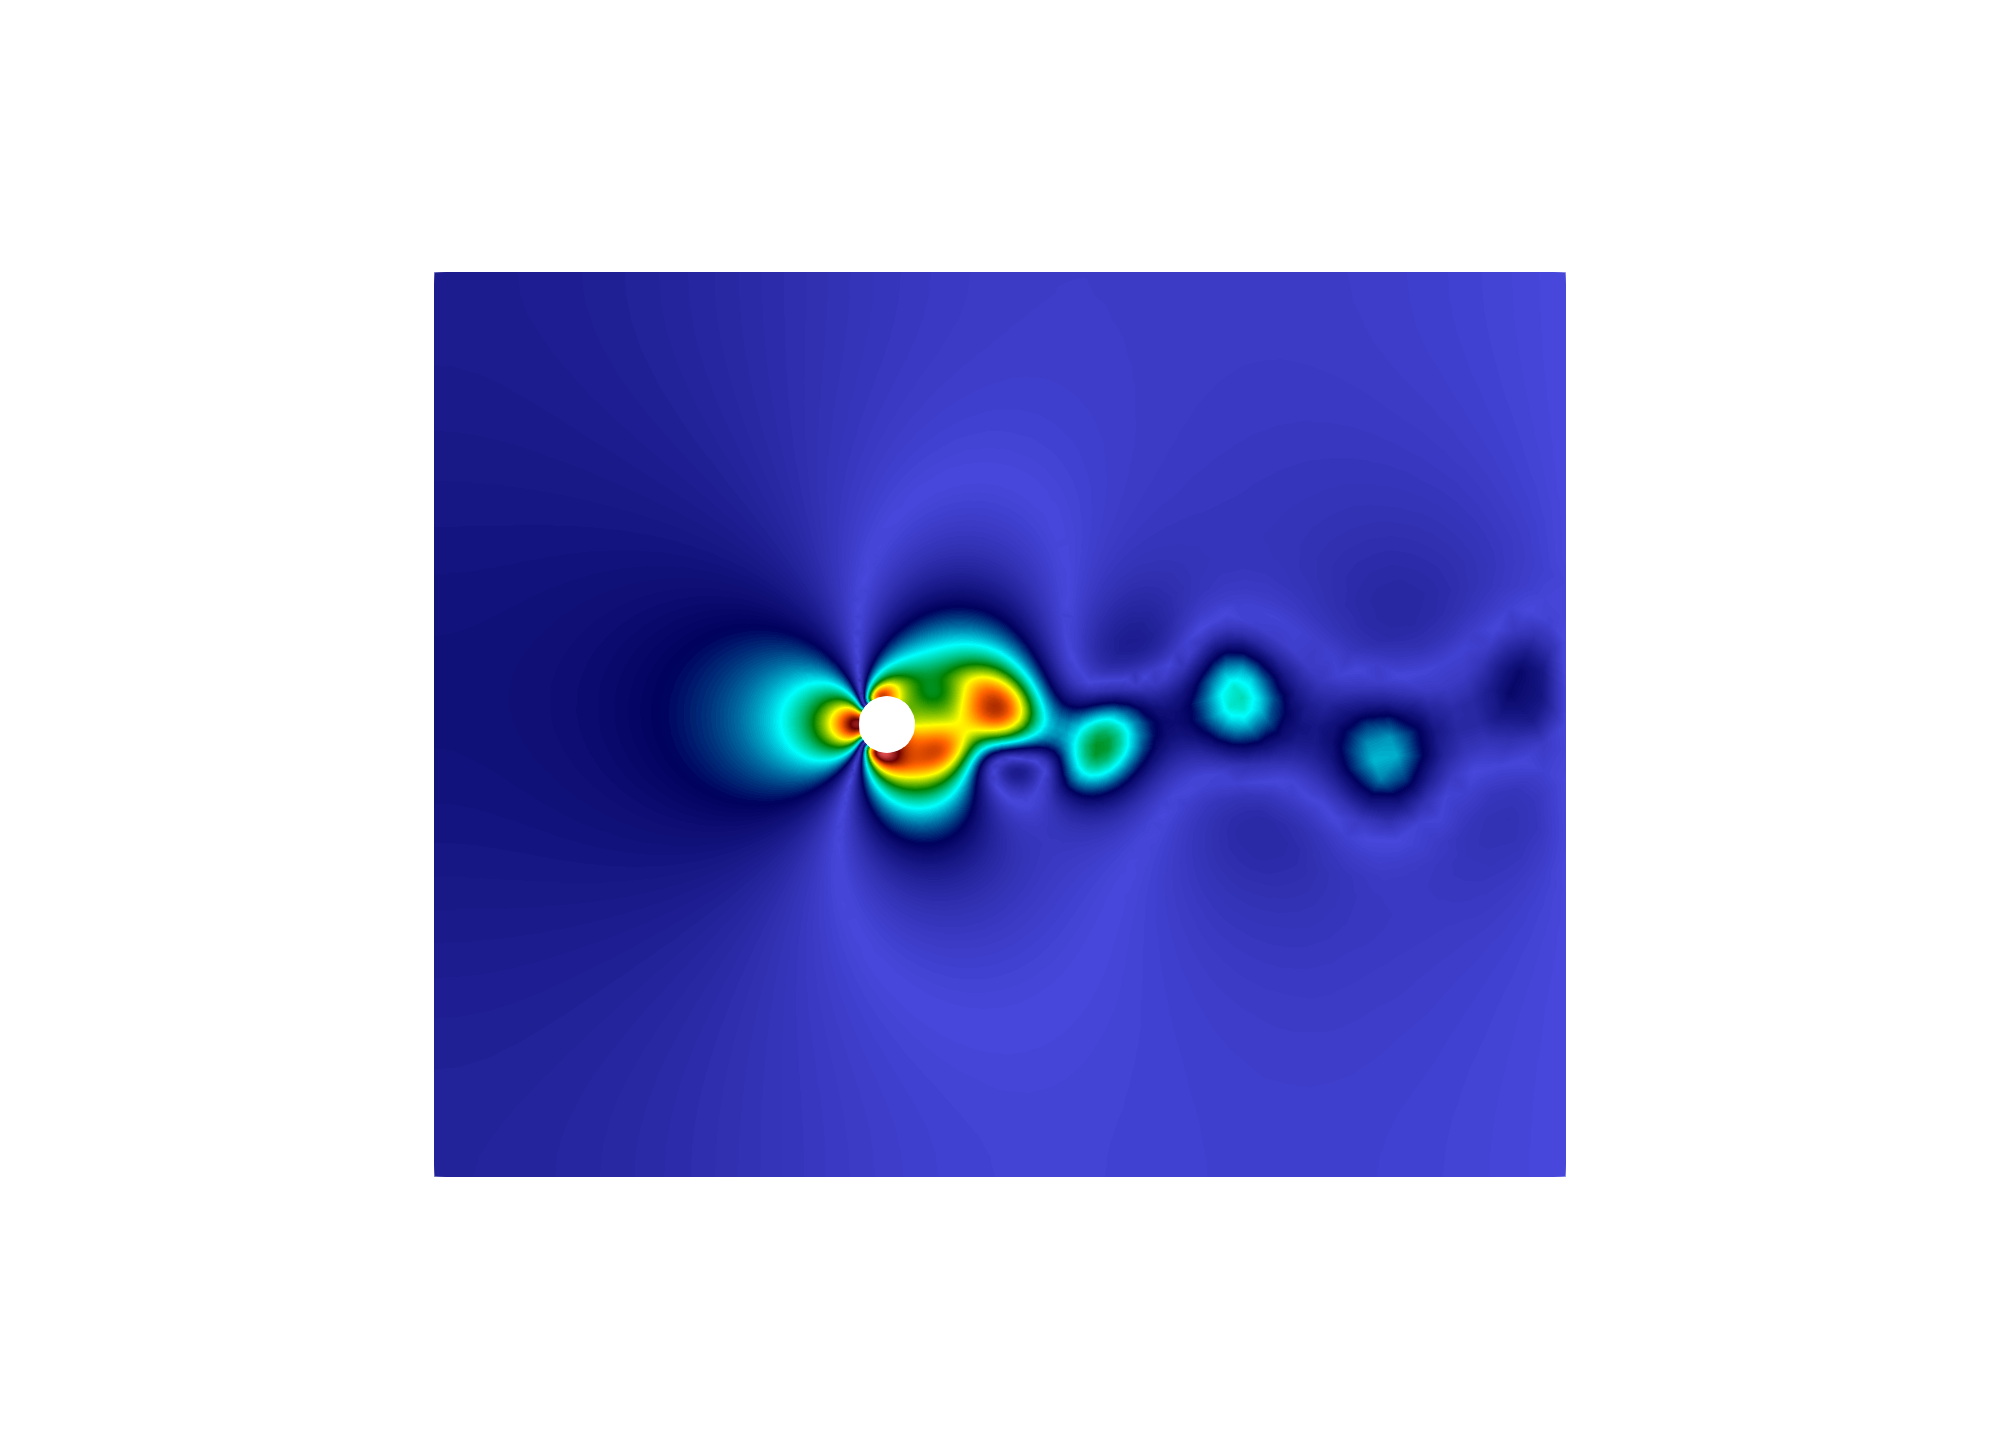
\includegraphics[scale=0.2,trim=15cm 9cm 14cm 9cm, clip=true]{Imagens/Cap2/pressaoRe100.png}}\\ 
	\subfloat[\label{fig:cilindro_2d_velocidade}Campo de velocidade]{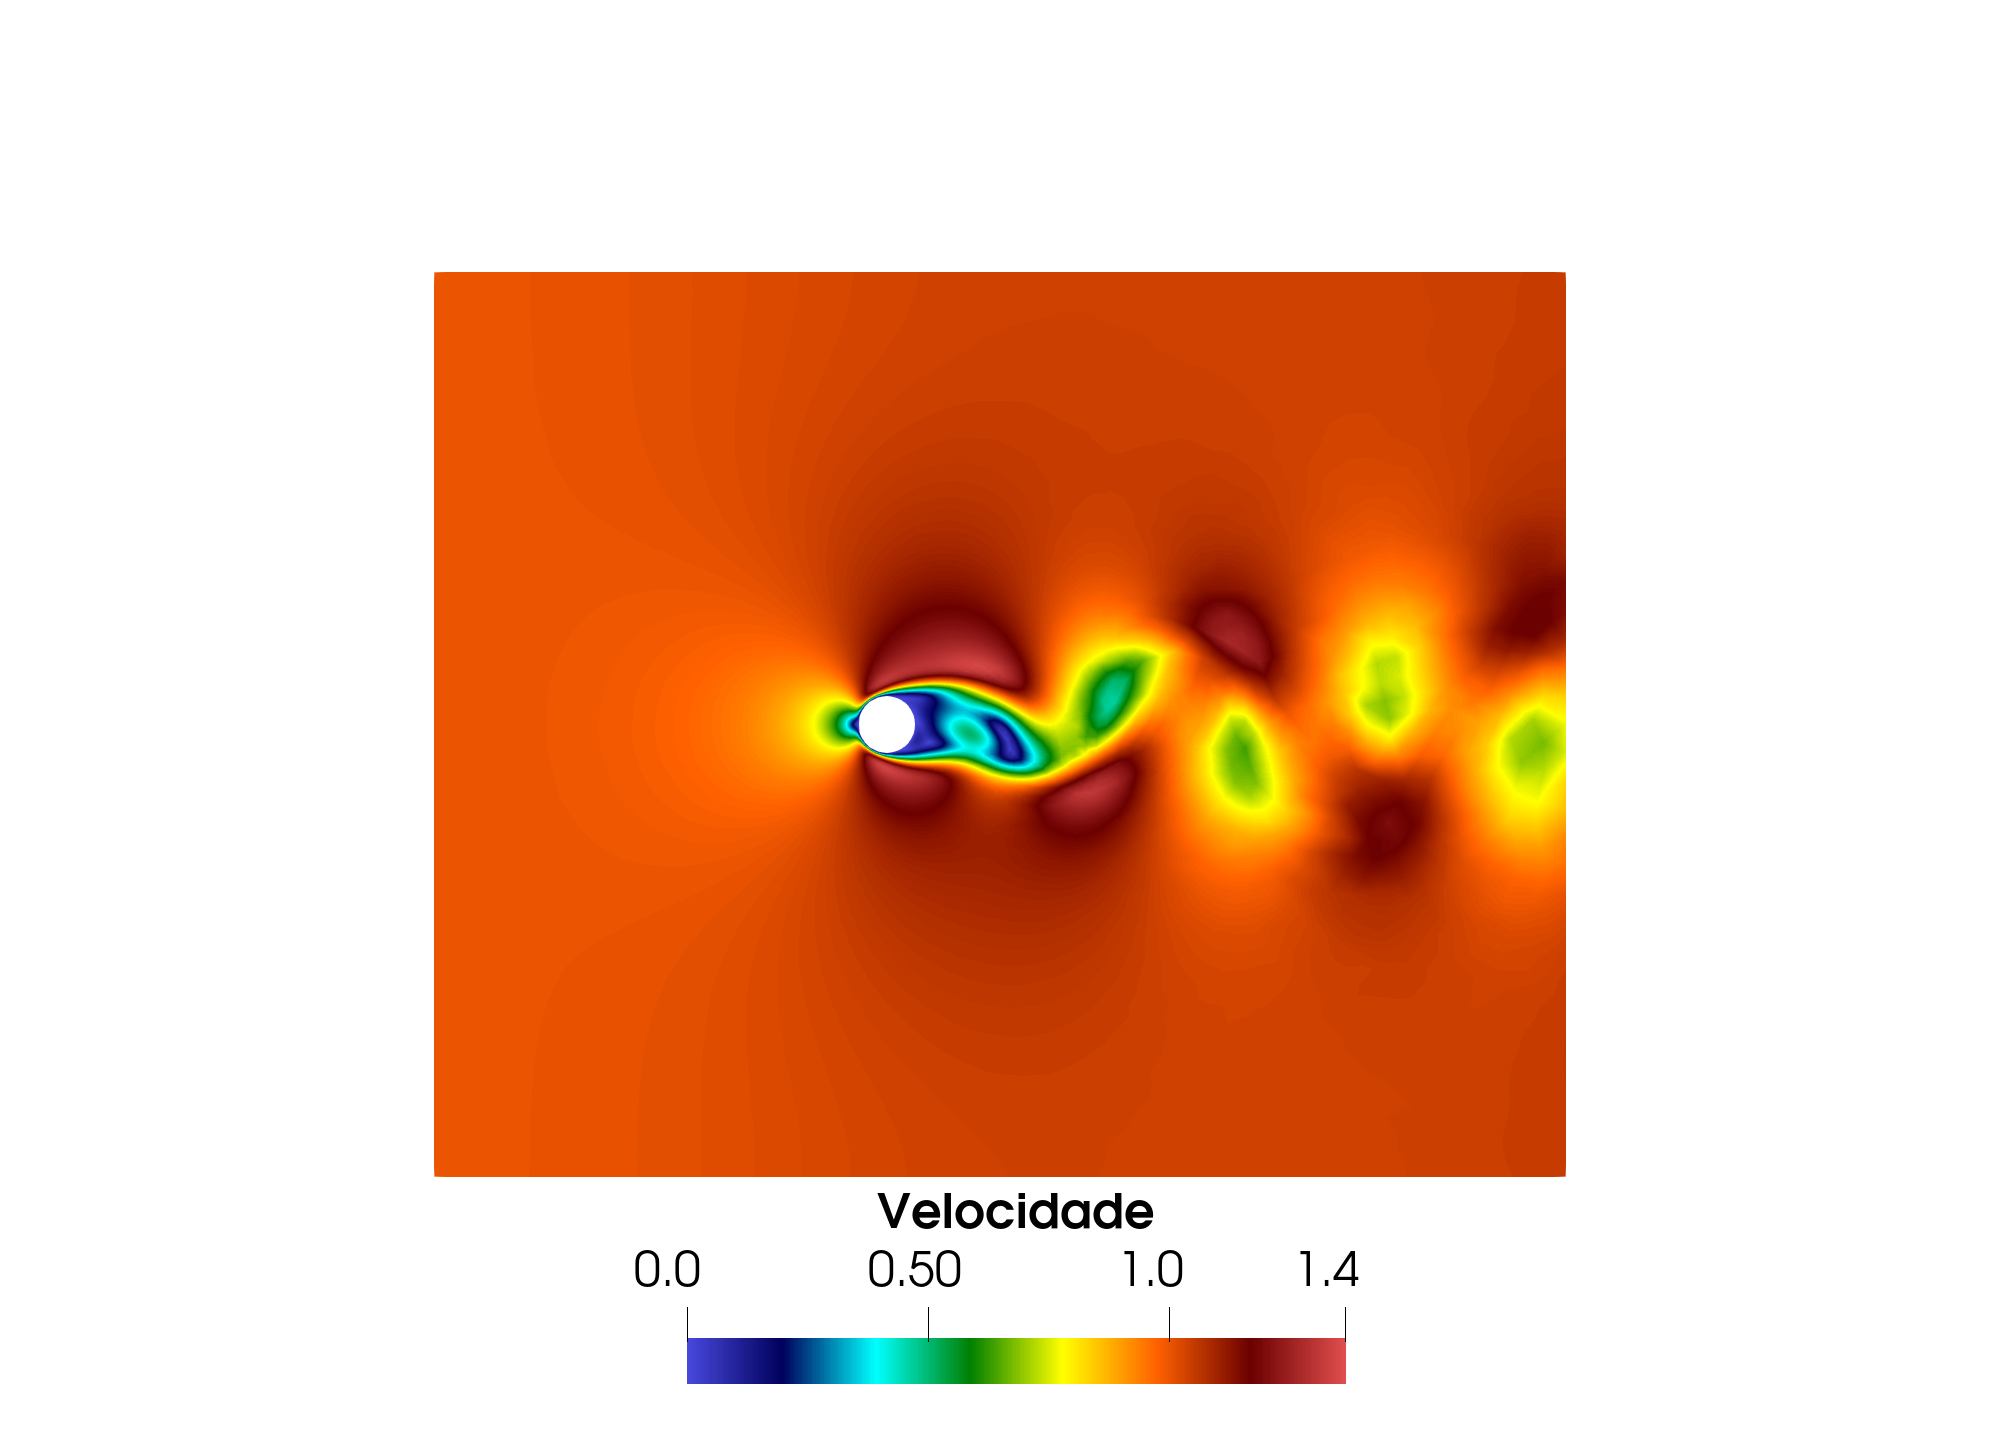
\includegraphics[scale=0.2,trim=15cm 1cm 14cm 9cm, clip=true]{Imagens/Cap2/velocitymagnitude.png}}
	\caption{Cilindro 2D: Campos de pressão e de velocidade para um escoamento com $Re = 100$ }
	\label{fig:cilindro_campos}
\end{figure}


\subsection{Cavidade Quadrada - 3D} \label{subsec:CavQua3d}

Para a verificação do código 3D utilizando elementos finitos o problema de uma cavidade quadrada com velocidade prescrita $u_{\infty}$ em sua parede superior foi estudado. A geometria do problema em questão e o conjunto de suas condições de contorno são apresentadas na Fig. \ref{fig:cavidade_geometria}. As paredes da cavidade são rígidas, com paredes laterais e do fundo com condição de aderência, e adicionalmente, velocidade $u_{z}=0$, condição de parede lisa, nas paredes das faces frontal e posterior. A cavidade possui na direção $z$ uma espessura de 0,03. A discretização espacial em elementos finitos utilizada é apresentada na Fig.  \ref{fig:cavidade_malha}, a qual consiste em 7252 elementos tetraédricos quadráticos e 14727 nós.

O problema é estudado para os números de Reynolds: 100, 400 e 1000. O número de Reynolds foi calculado de acordo com Eq. \eqref{eq:Reynolds}, com $L$ equivalente ao comprimento do lado da cavidade. O problema foi simulado para uma velocidade na parede superior de $\velocity_{\infty} = 1,0$, $\rho = 1,0$, $\timeStep = 0,05$, e $\specRadius = 0$, sendo a viscosidade do fluido variada de modo a alterar o número de Reynolds. A simulação foi mantida até que se atingiu o estado estacionário de escoamento. 

\begin{figure}[!htb]
	\centering
	\subfloat[Geometria e condições de contorno.\label{fig:cavidade_geometria}]{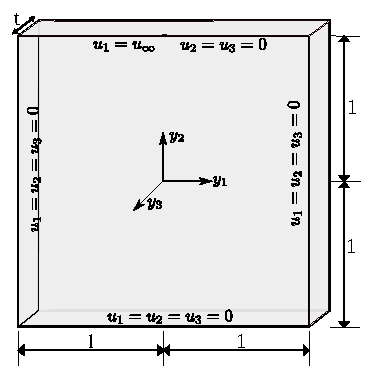
\includegraphics[scale=1.0,trim=0cm 0cm 0cm 0cm, clip=true]{Imagens/Cap2/cavidade.pdf}} \quad
	\subfloat[Discretização espacial.\label{fig:cavidade_malha}]{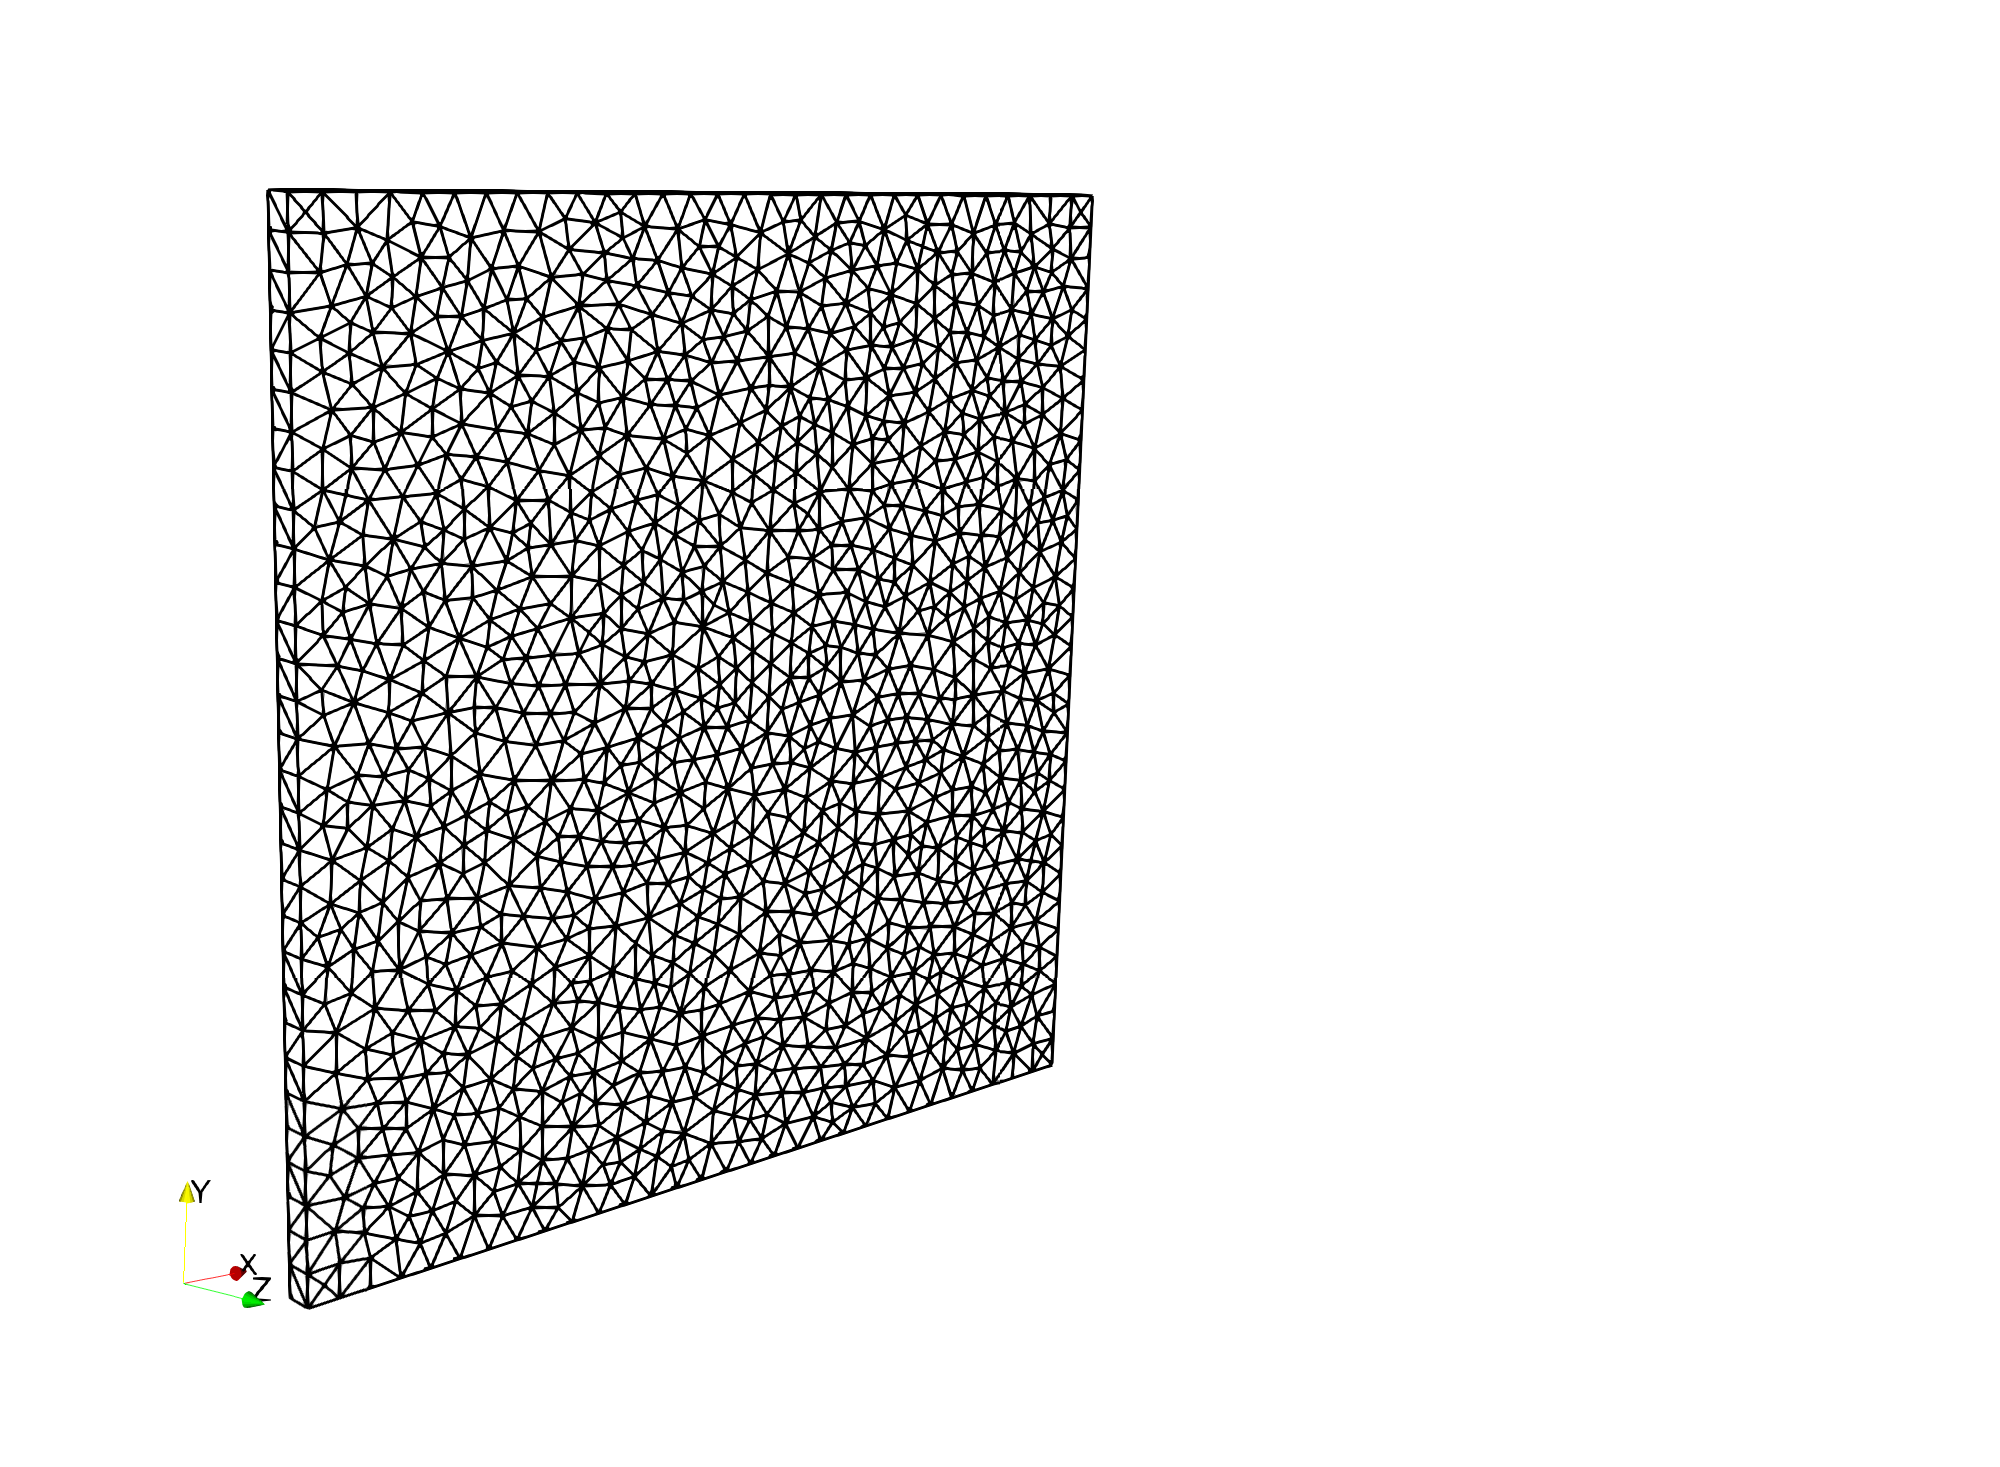
\includegraphics[trim=170 120 850 130,clip,scale=0.15]{Imagens/Cap2/cavitymesh.png}}
	\caption{Cavidade quadrada: Geometria, condições de contorno e malha de elementos finitos.}
\end{figure}

Os perfis de velocidade adimensionalizados ($\velocity/\velocinfty$) horizontal e vertical ao longo de duas linhas centrais nas direções $x$ e $y$ posicionadas no centro da espessura na direção $z$ da cavidade são apresentados na Fig. \ref{fig:cavidade_graficos} e comparados com a referência de \citeonline{GhiaGS:1982}.


\begin{figure}[!t]
	\centering
	\subfloat[\label{fig:cavidade_g_Re100}$Re$=100.]{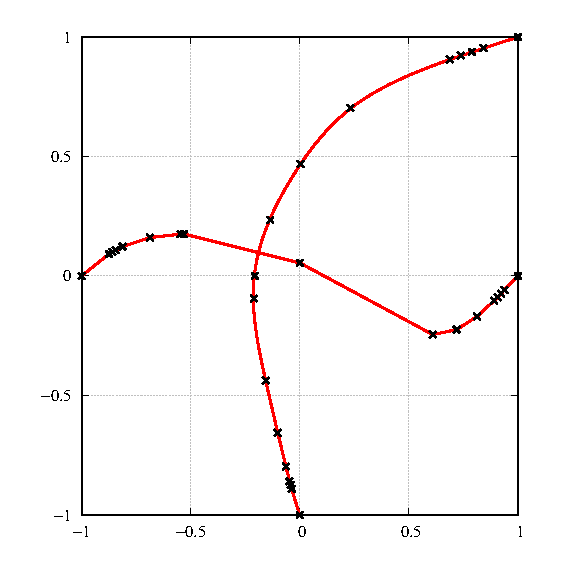
\includegraphics[scale=.8,trim=0.55cm 0.5cm 0.3cm 0.2cm, clip=true]{Imagens/Cap2/cavidade_Re100.eps}} \subfloat[\label{fig:cavidade_g_Re400}$Re$=400.]{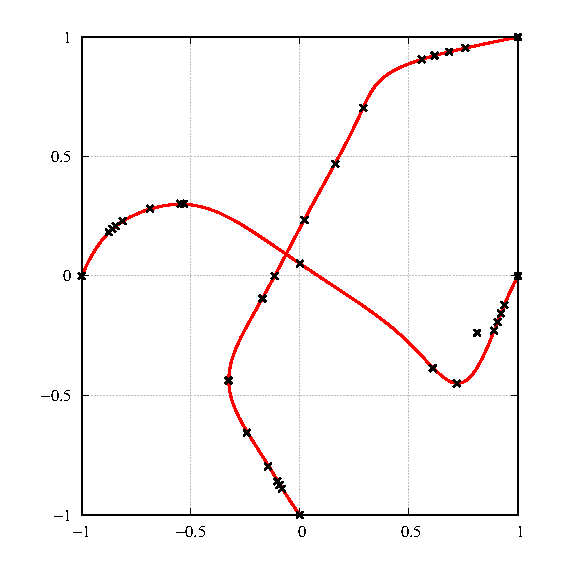
\includegraphics[scale=.8,trim=0.55cm 0.5cm 0.3cm 0.2cm, clip=true]{Imagens/Cap2/cavidade_Re400.eps}}\\ 
	\subfloat[\label{fig:cavidade_g_Re1000}$Re$=1000.]{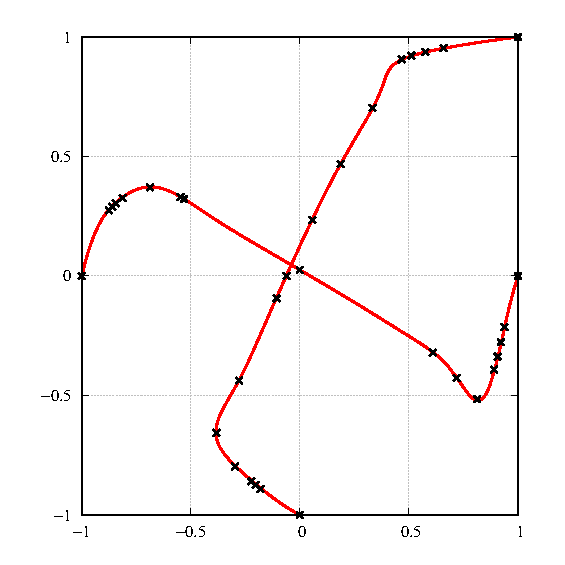
\includegraphics[scale=.8,trim=0.55cm 0.5cm 0.3cm 0.2cm, clip=true]{Imagens/Cap2/cavidade_Re1000.eps}} \\
	\subfloat{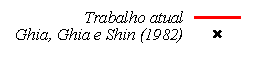
\includegraphics[scale=1.]{Imagens/Cap2/legenda.pdf}} 
	\caption{Cavidade quadrada: Perfis de velocidade adimensionalizados nas direções $x$ e $y$ . }
	\label{fig:cavidade_graficos}
\end{figure}

Os campos de velocidade e de pressão são apresentados nas figuras Fig \ref{fig:cav3d-vel} e \ref{fig:cav3d-press} respectivamente. Ressalta-se que para a solução do problema, por se tratar de um problema com todos os contornos com condição de Dirichlet impostos, a pressão torna-se indefinida. Por esse motivo, prescreveu-se uma pressão $\press = \press_{ref} =  0$ no canto superior direito da cavidade. 


\begin{figure}[!t]
	\centering
	\setlength{\lineskip}{-10pt}
	\subfloat[\label{fig:cavidade_Vel_Re100}$Re$=100.]{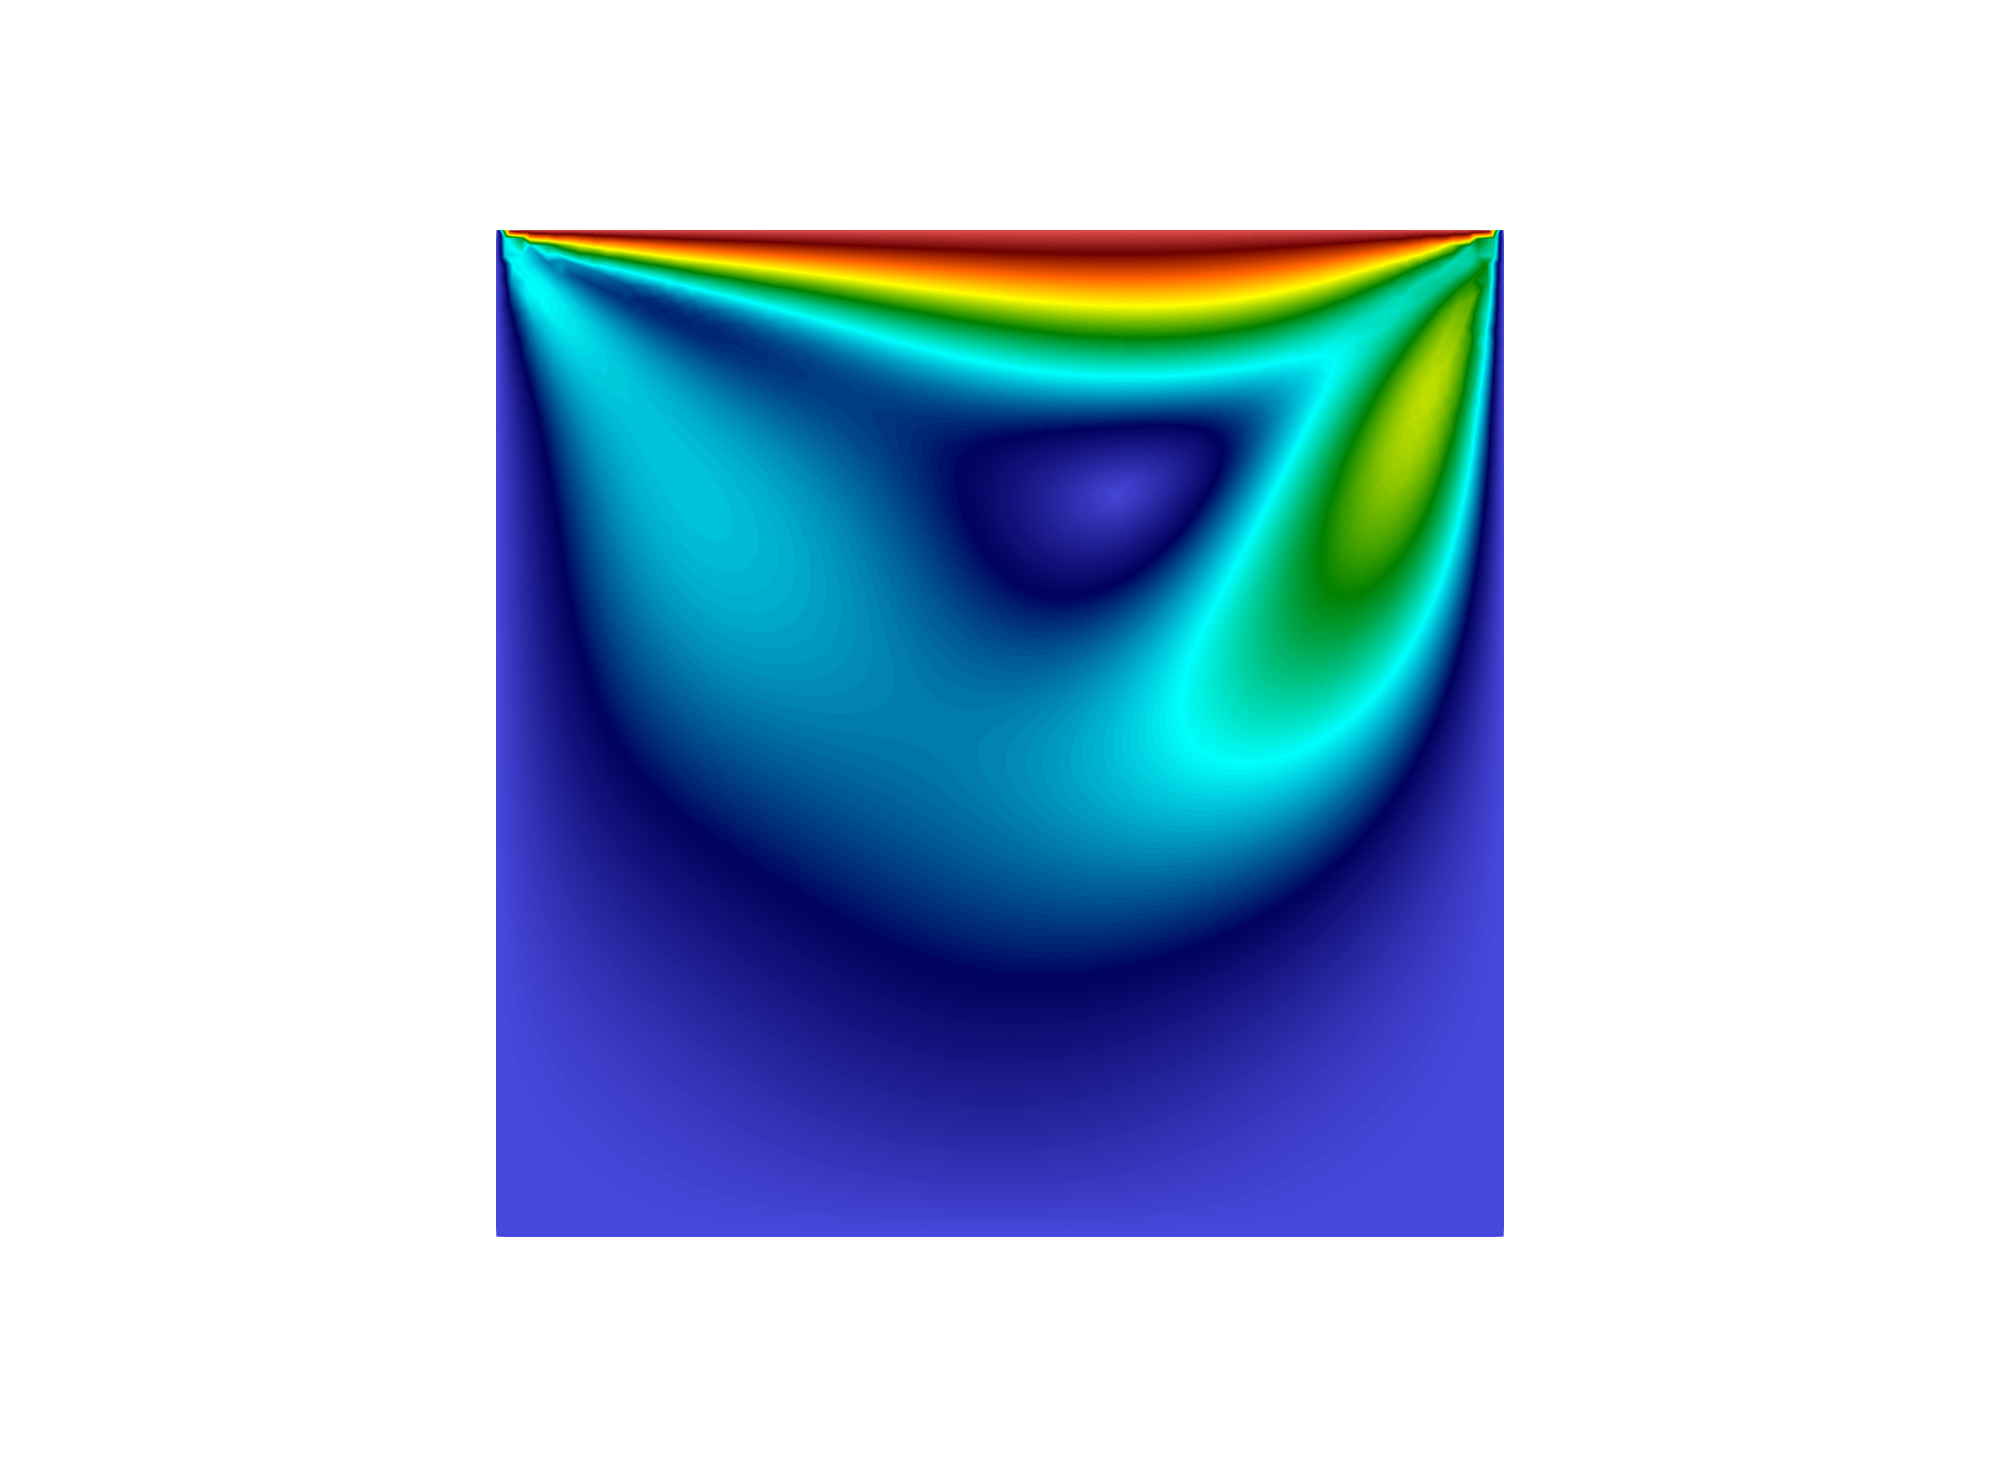
\includegraphics[scale=0.15,trim=15cm 7cm 15cm 7cm, clip=true]{Imagens/Cap2/velocity-Re100.png}} \subfloat[\label{fig:cavidade_Vel_Re400}$Re$=400.]{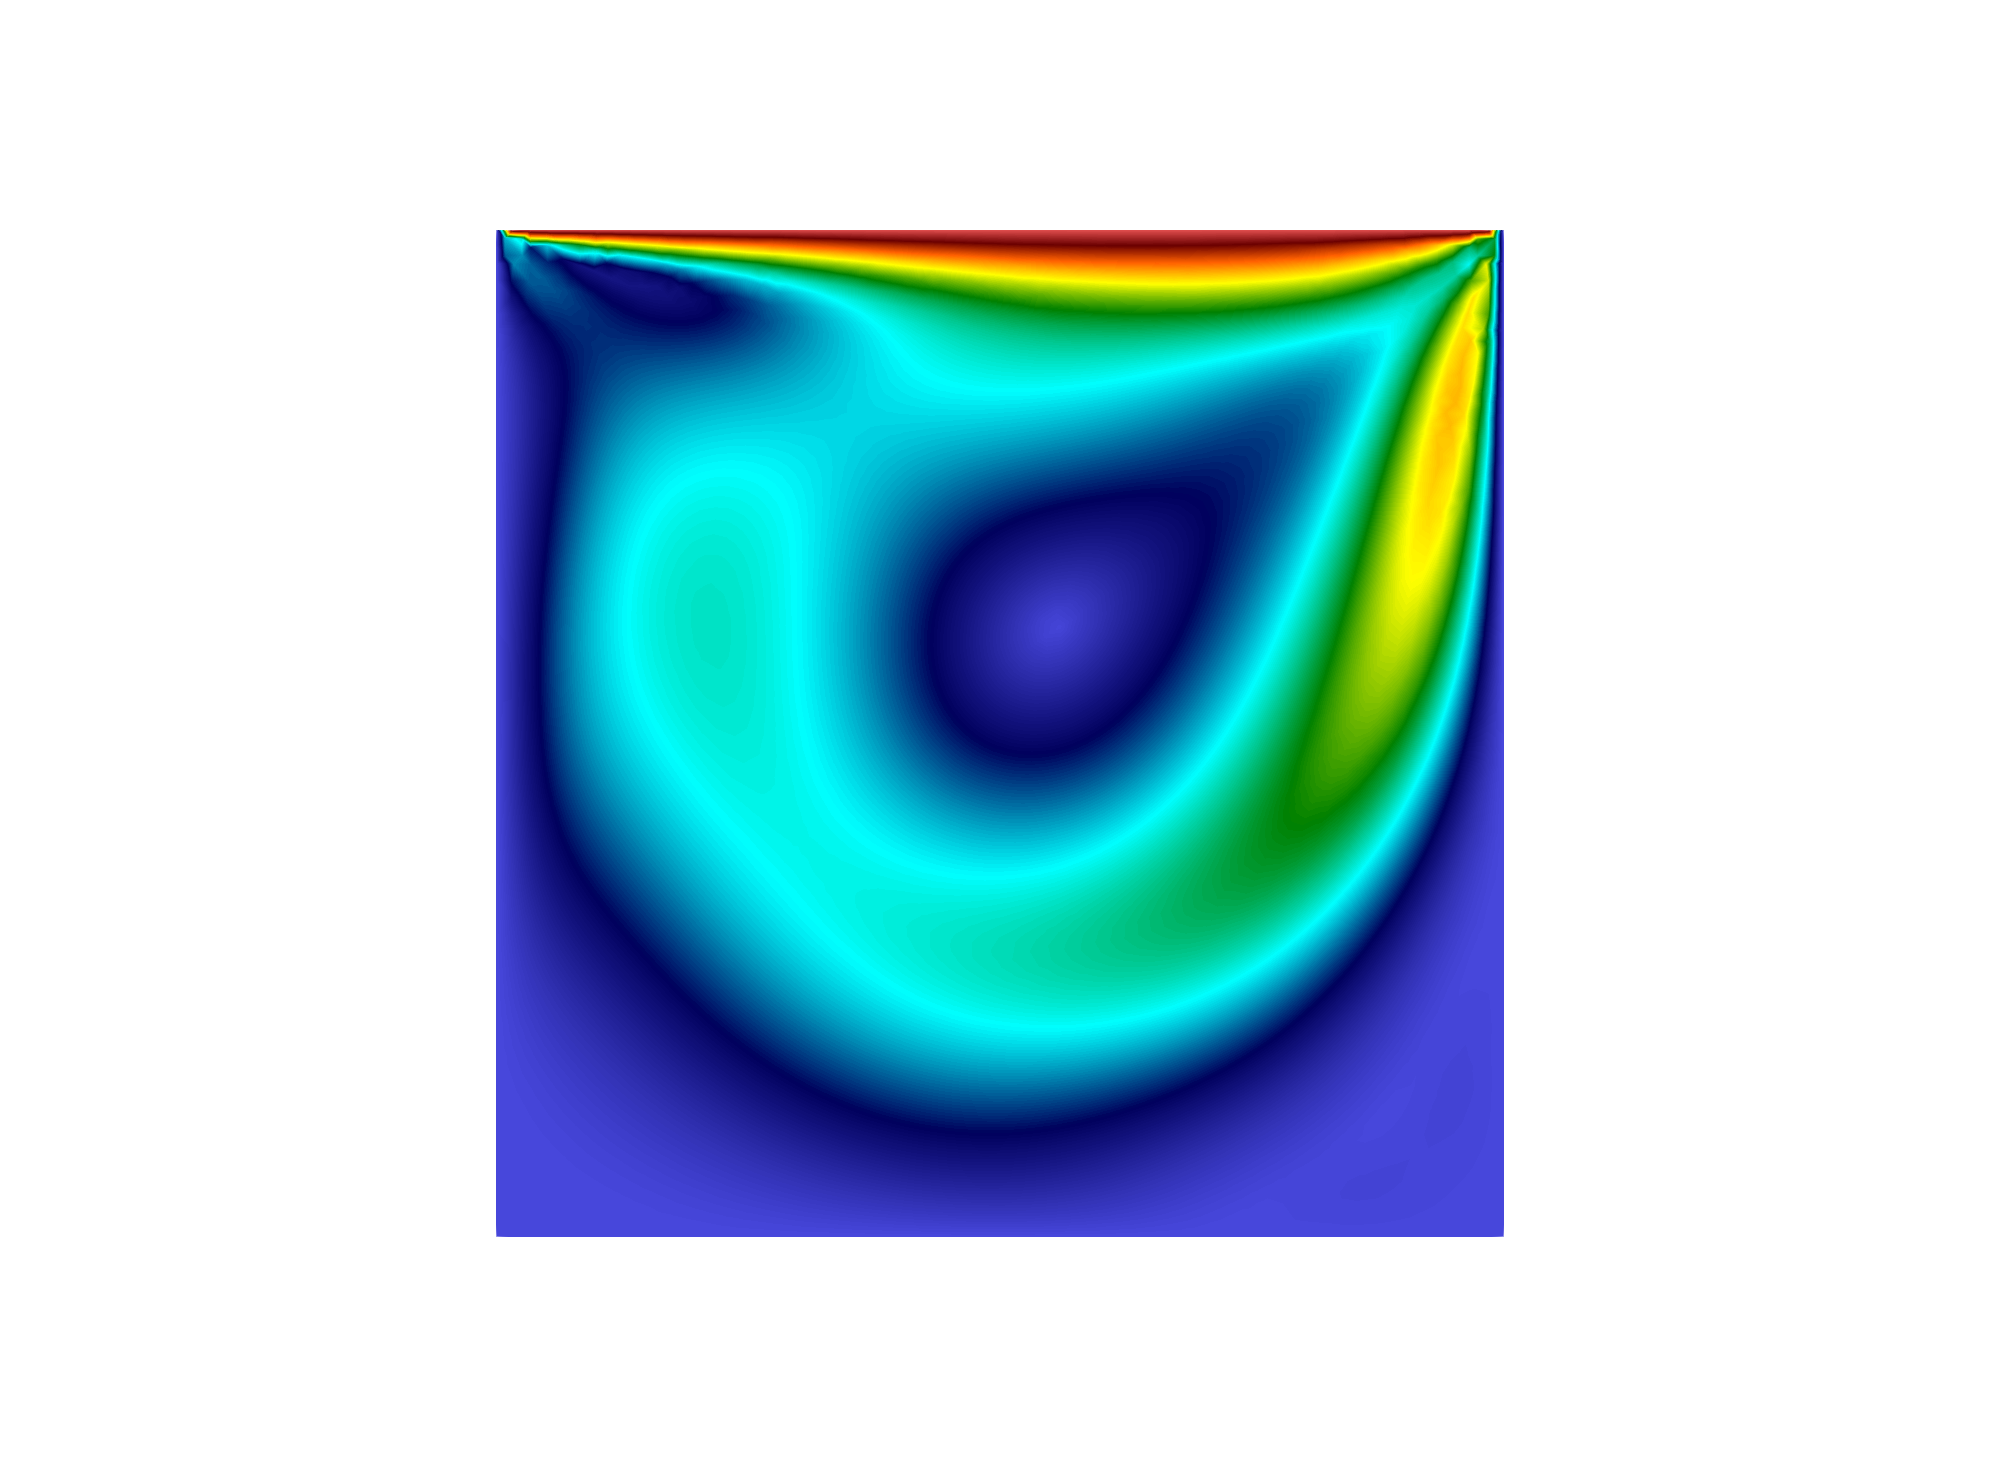
\includegraphics[scale=0.15,trim=15cm 7cm 15cm 7cm, clip=true]{Imagens/Cap2/velocity-Re400.png}}\\ 
	\subfloat[\label{fig:cavidade_Vel_Re1000}$Re$=1000.]{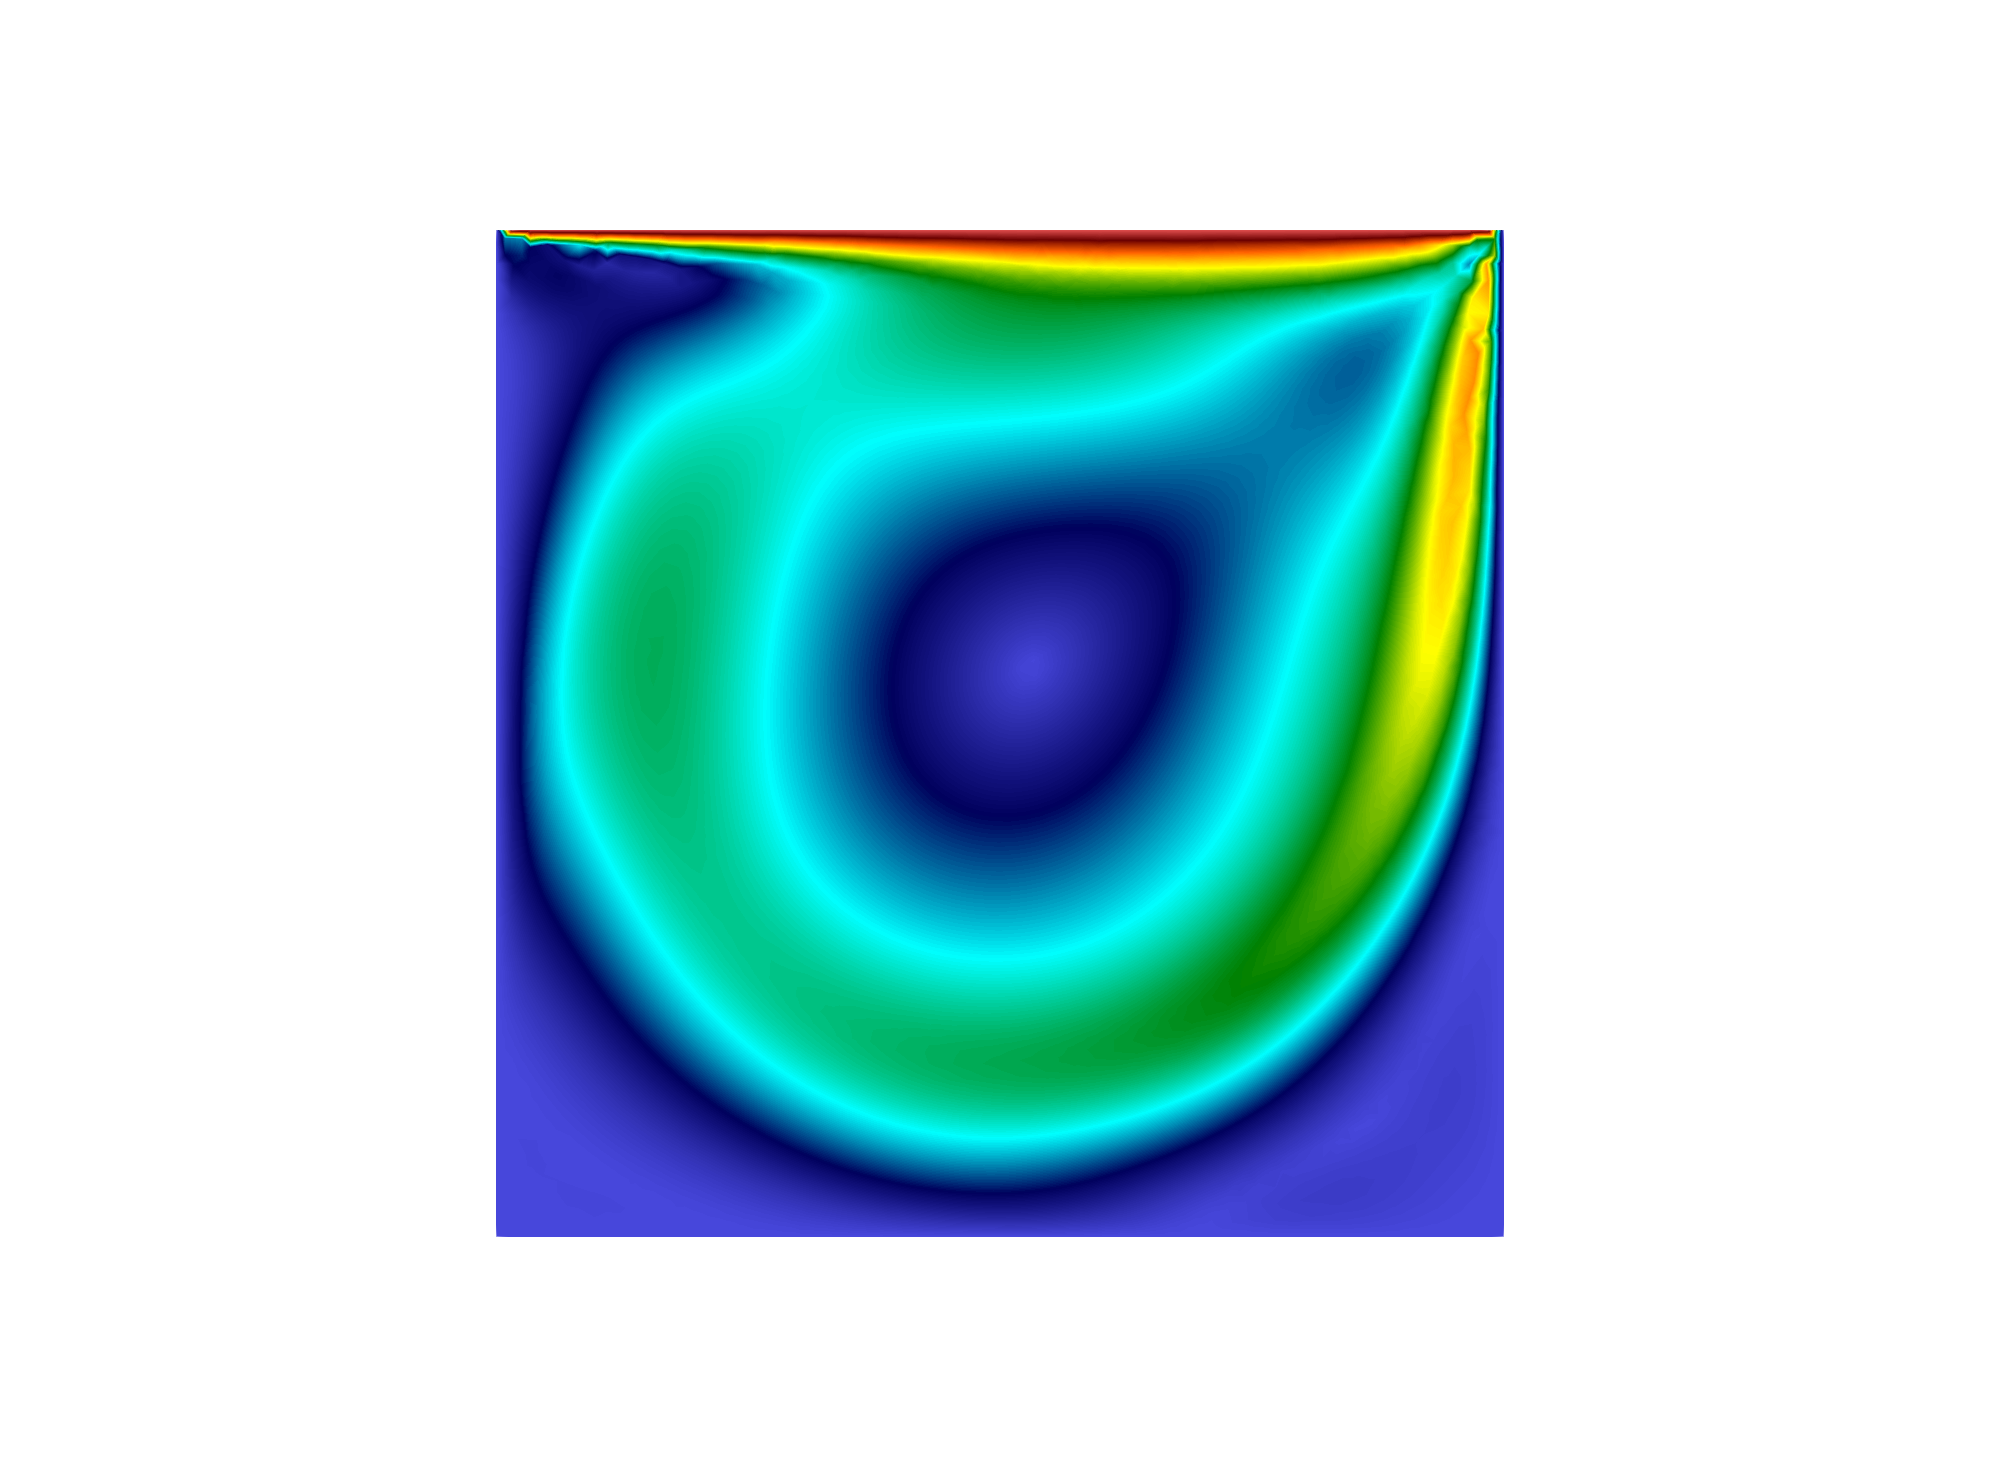
\includegraphics[scale=0.15,trim=15cm 7cm 15cm 7cm, clip=true]{Imagens/Cap2/velocity-Re1000.png}} \\
	%	\subfloat[\label{fig:cavidade_g_Re10000}$Re$=10000.]{\includegraphics[scale=1.1,trim=0.55cm 0.5cm 0.3cm 0.2cm, clip=true]{Imagens/Cap2/cavidade_Re10000.eps}}\\
	\subfloat{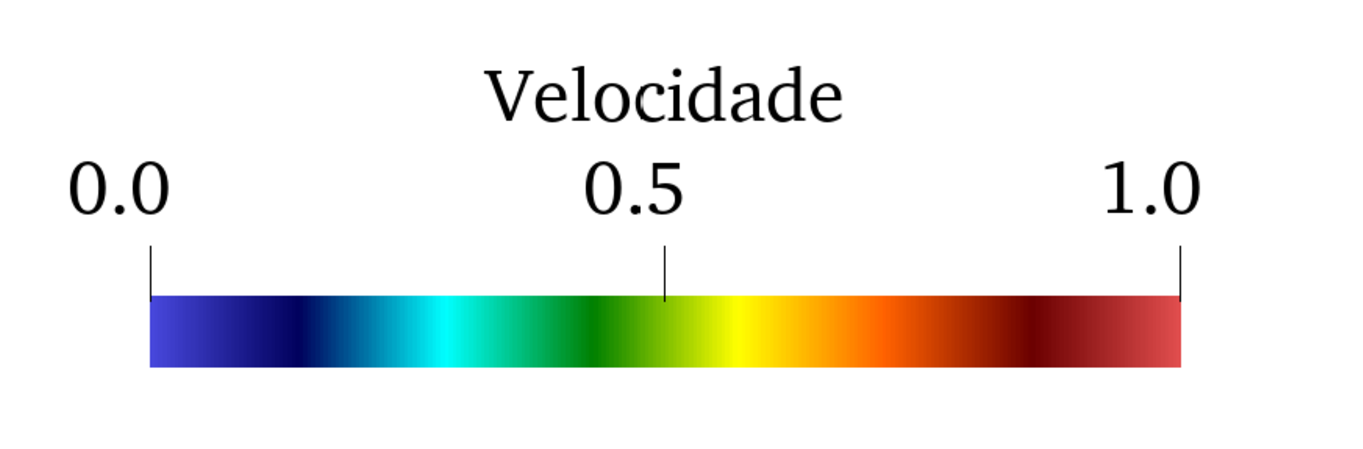
\includegraphics[scale=0.2]{Imagens/Cap2/legandaCavidadeVel.pdf}} 
	\caption{Cavidade quadrada: campos de velocidade. }
	\label{fig:cav3d-vel}
\end{figure}

\begin{figure}[!t]
	\centering
	\setlength{\lineskip}{-10pt}
	\subfloat[\label{fig:cavidade_Press_Re100}$Re$=100.]{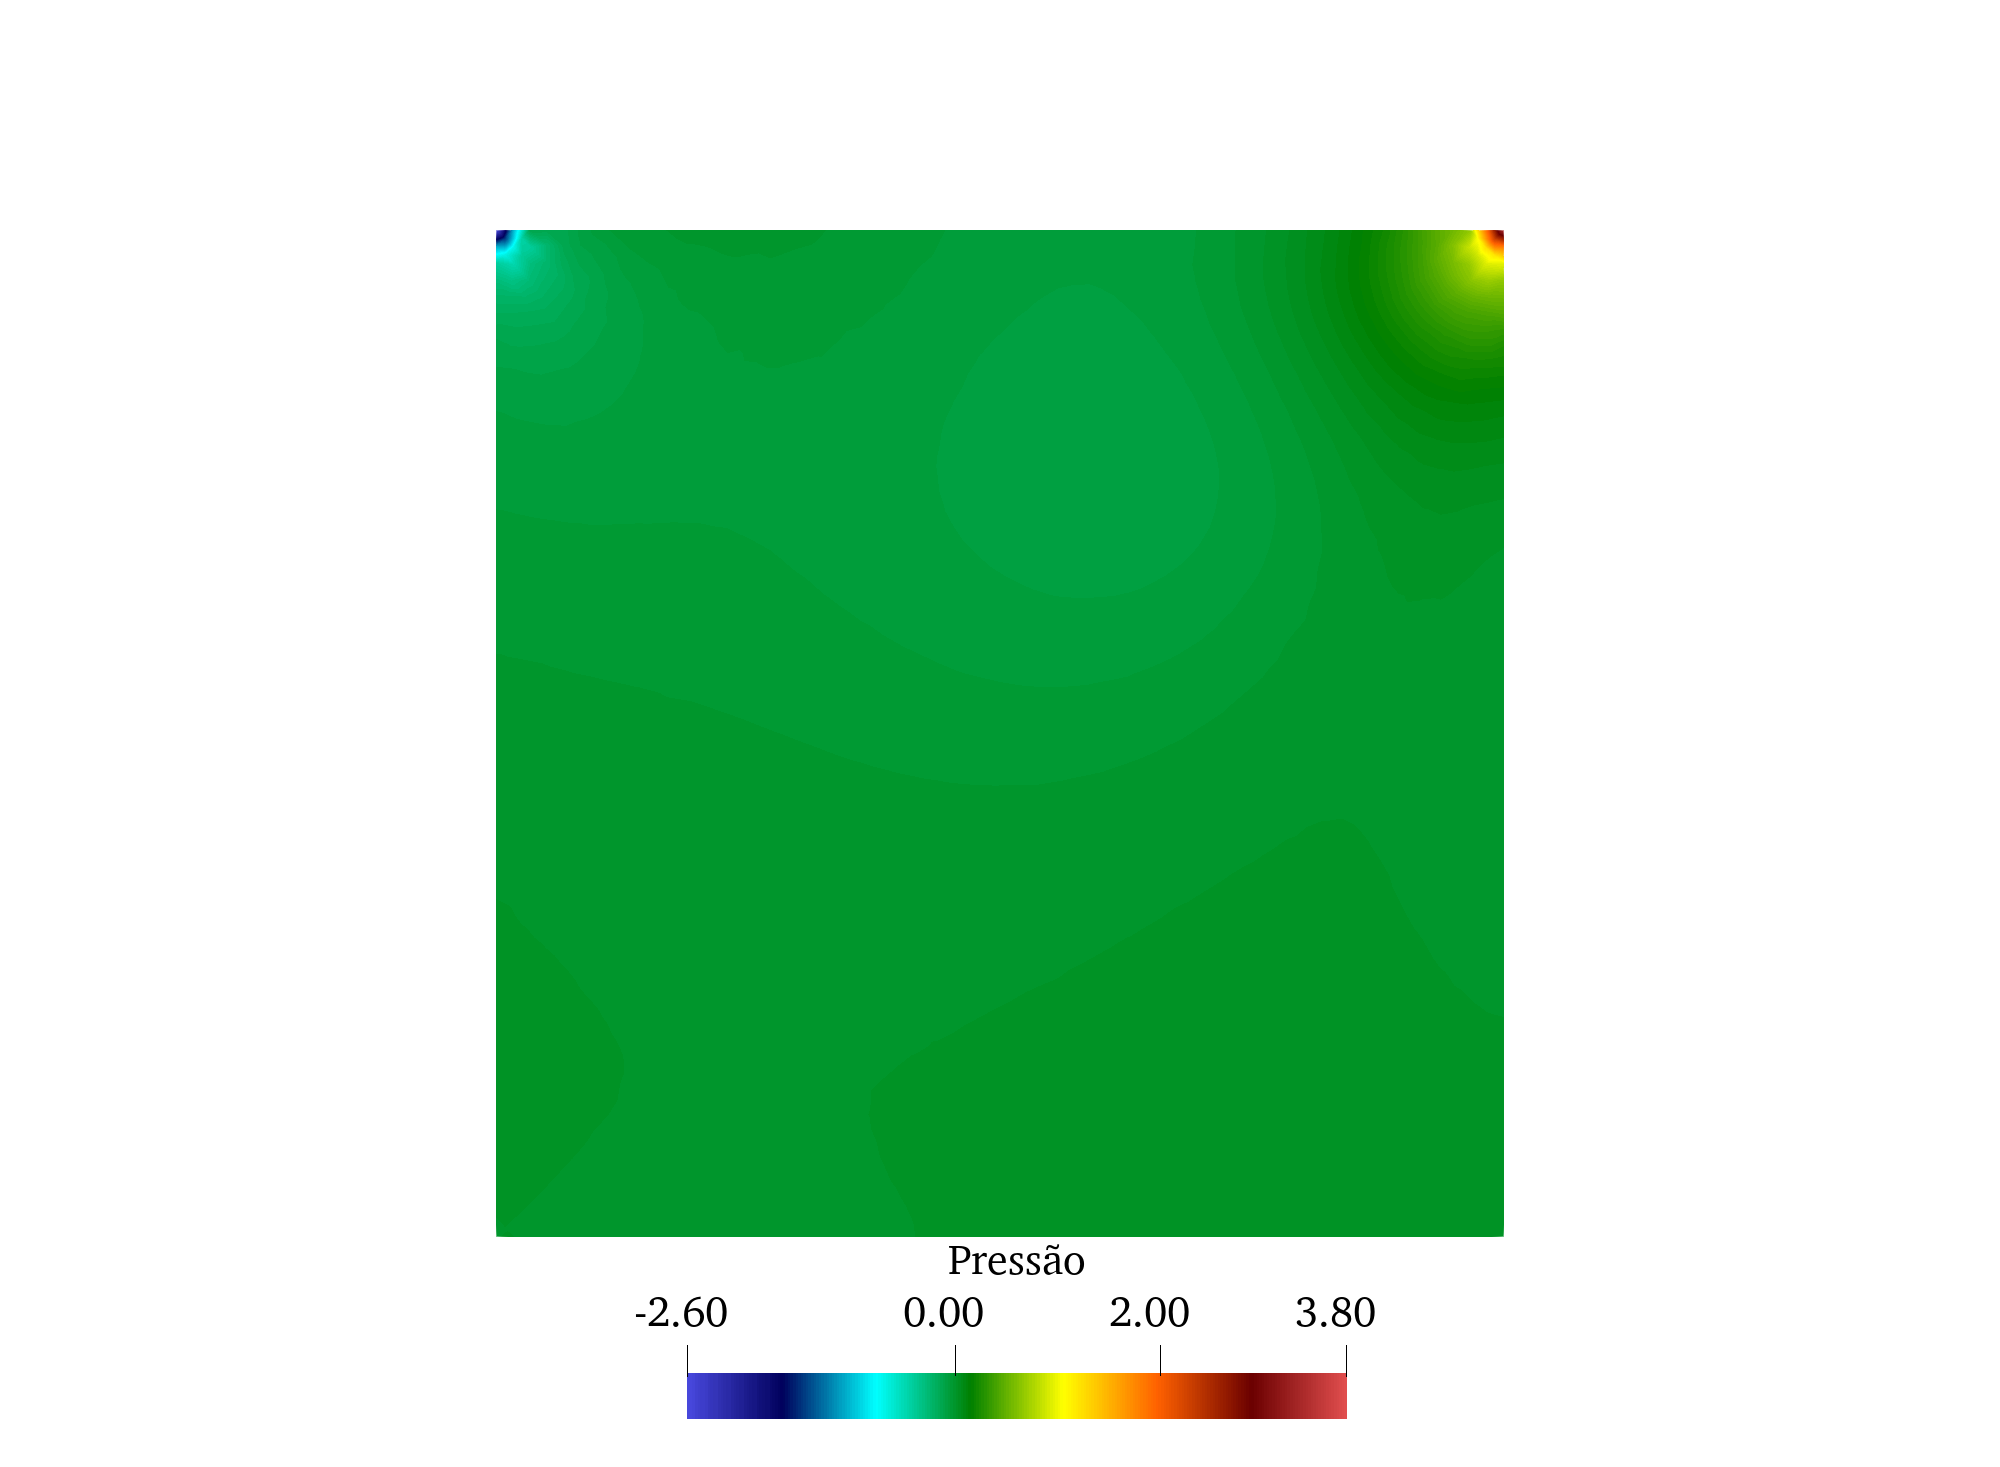
\includegraphics[scale=0.15,trim=15cm 0cm 15cm 7cm, clip=true]{Imagens/Cap2/pressao100.png}} \subfloat[\label{fig:cavidade_Press_Re400}$Re$=400.]{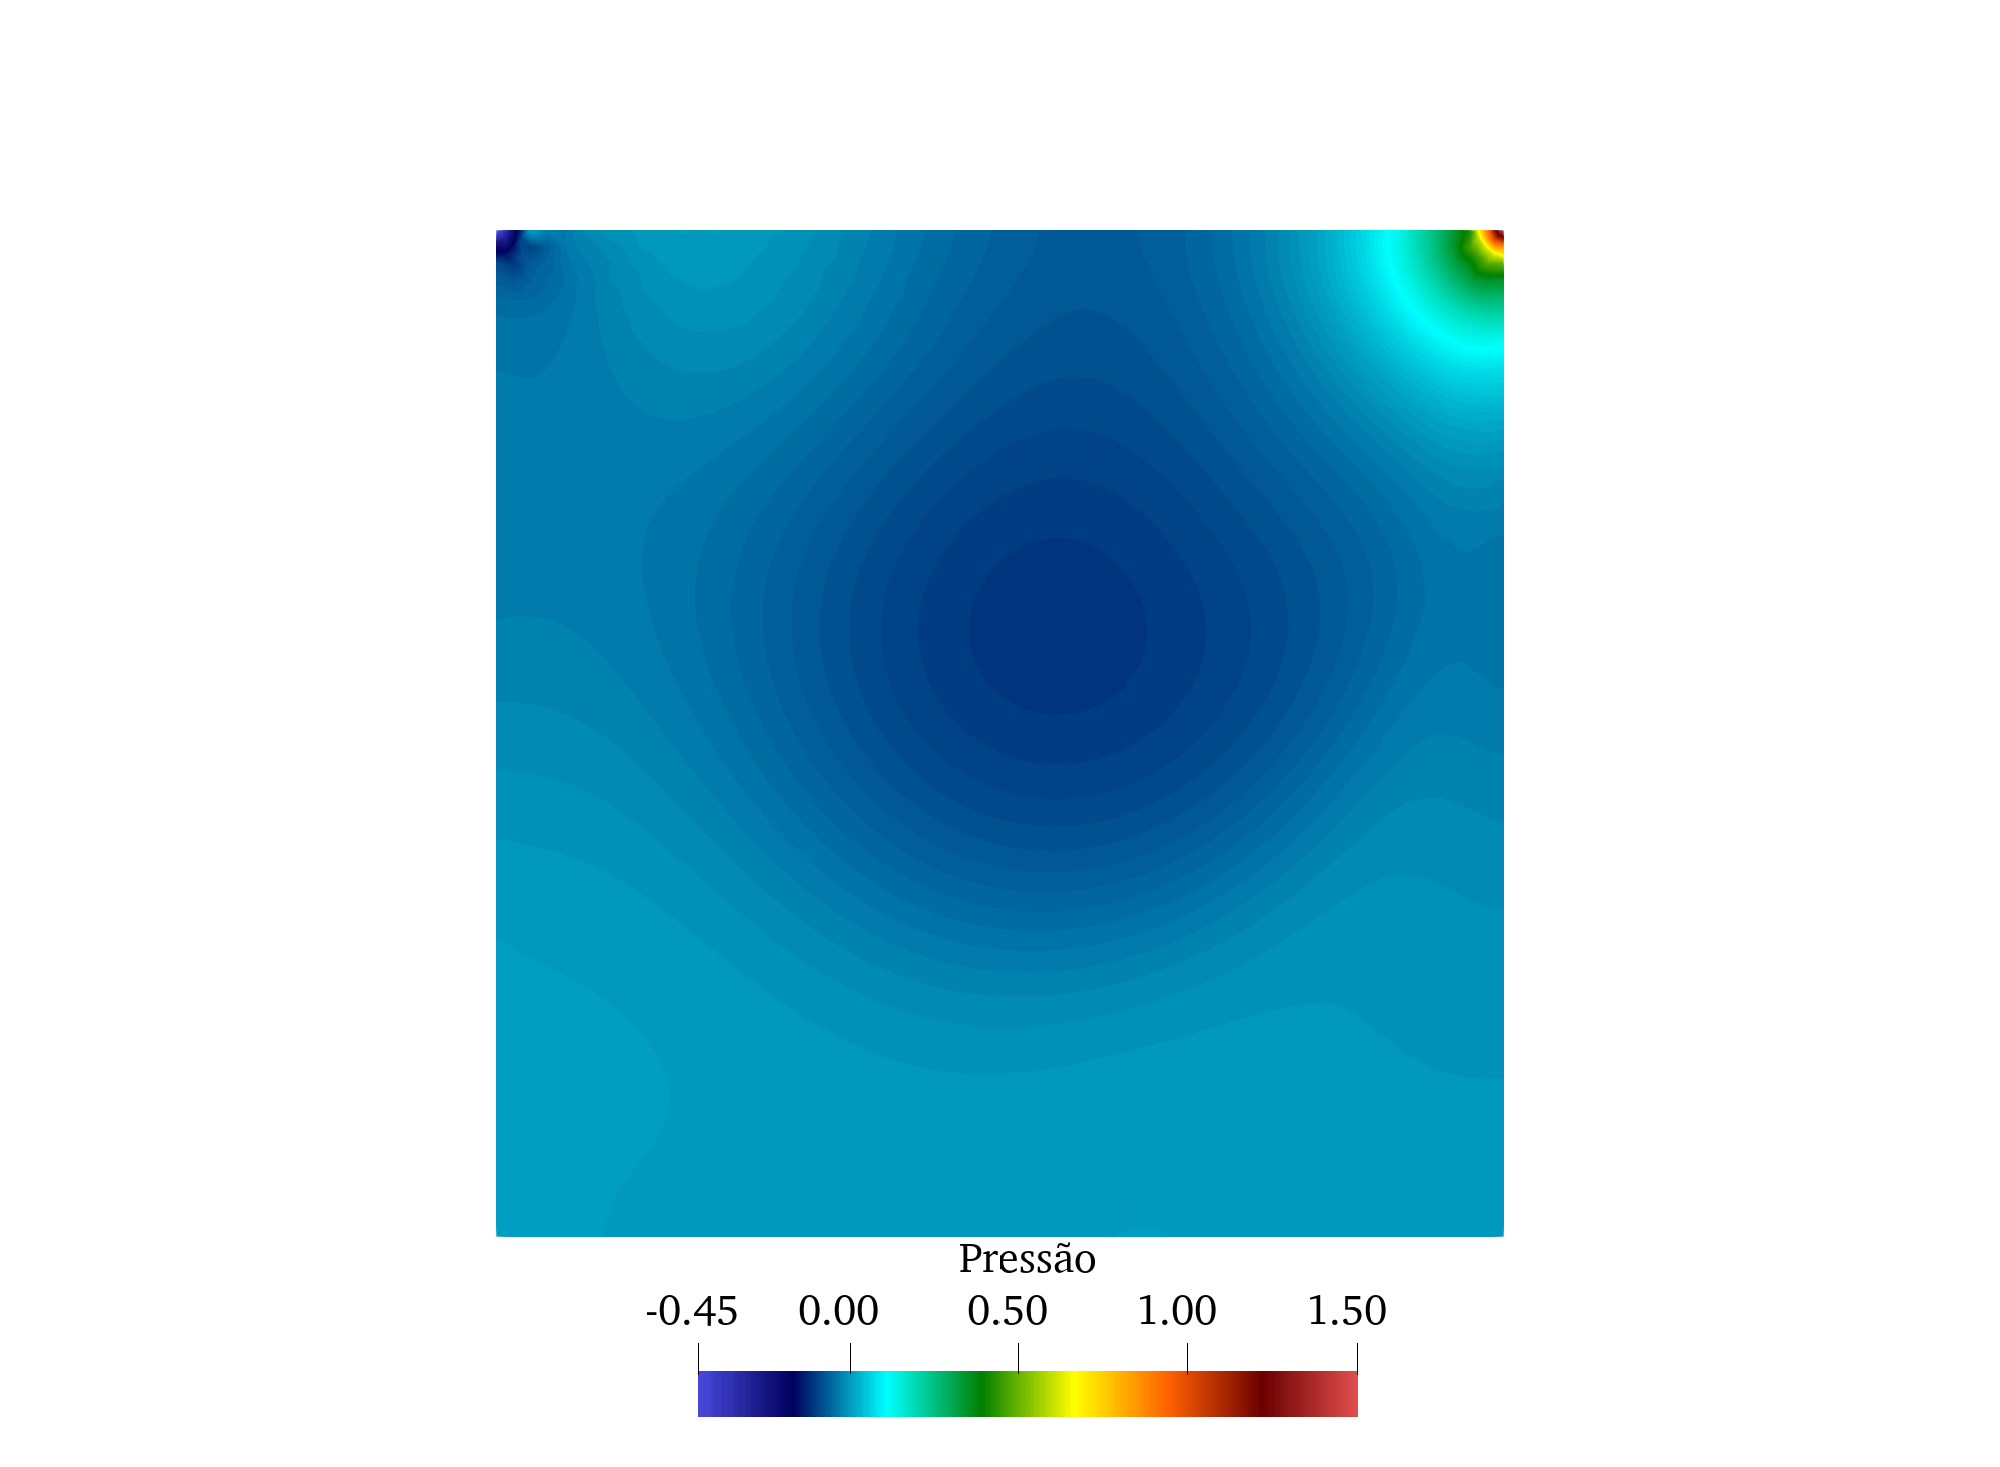
\includegraphics[scale=0.15,trim=15cm 0cm 15cm 7cm, clip=true]{Imagens/Cap2/pressao400.png}}\\ 
	\subfloat[\label{fig:cavidade_Press_Re1000}$Re$=1000.]{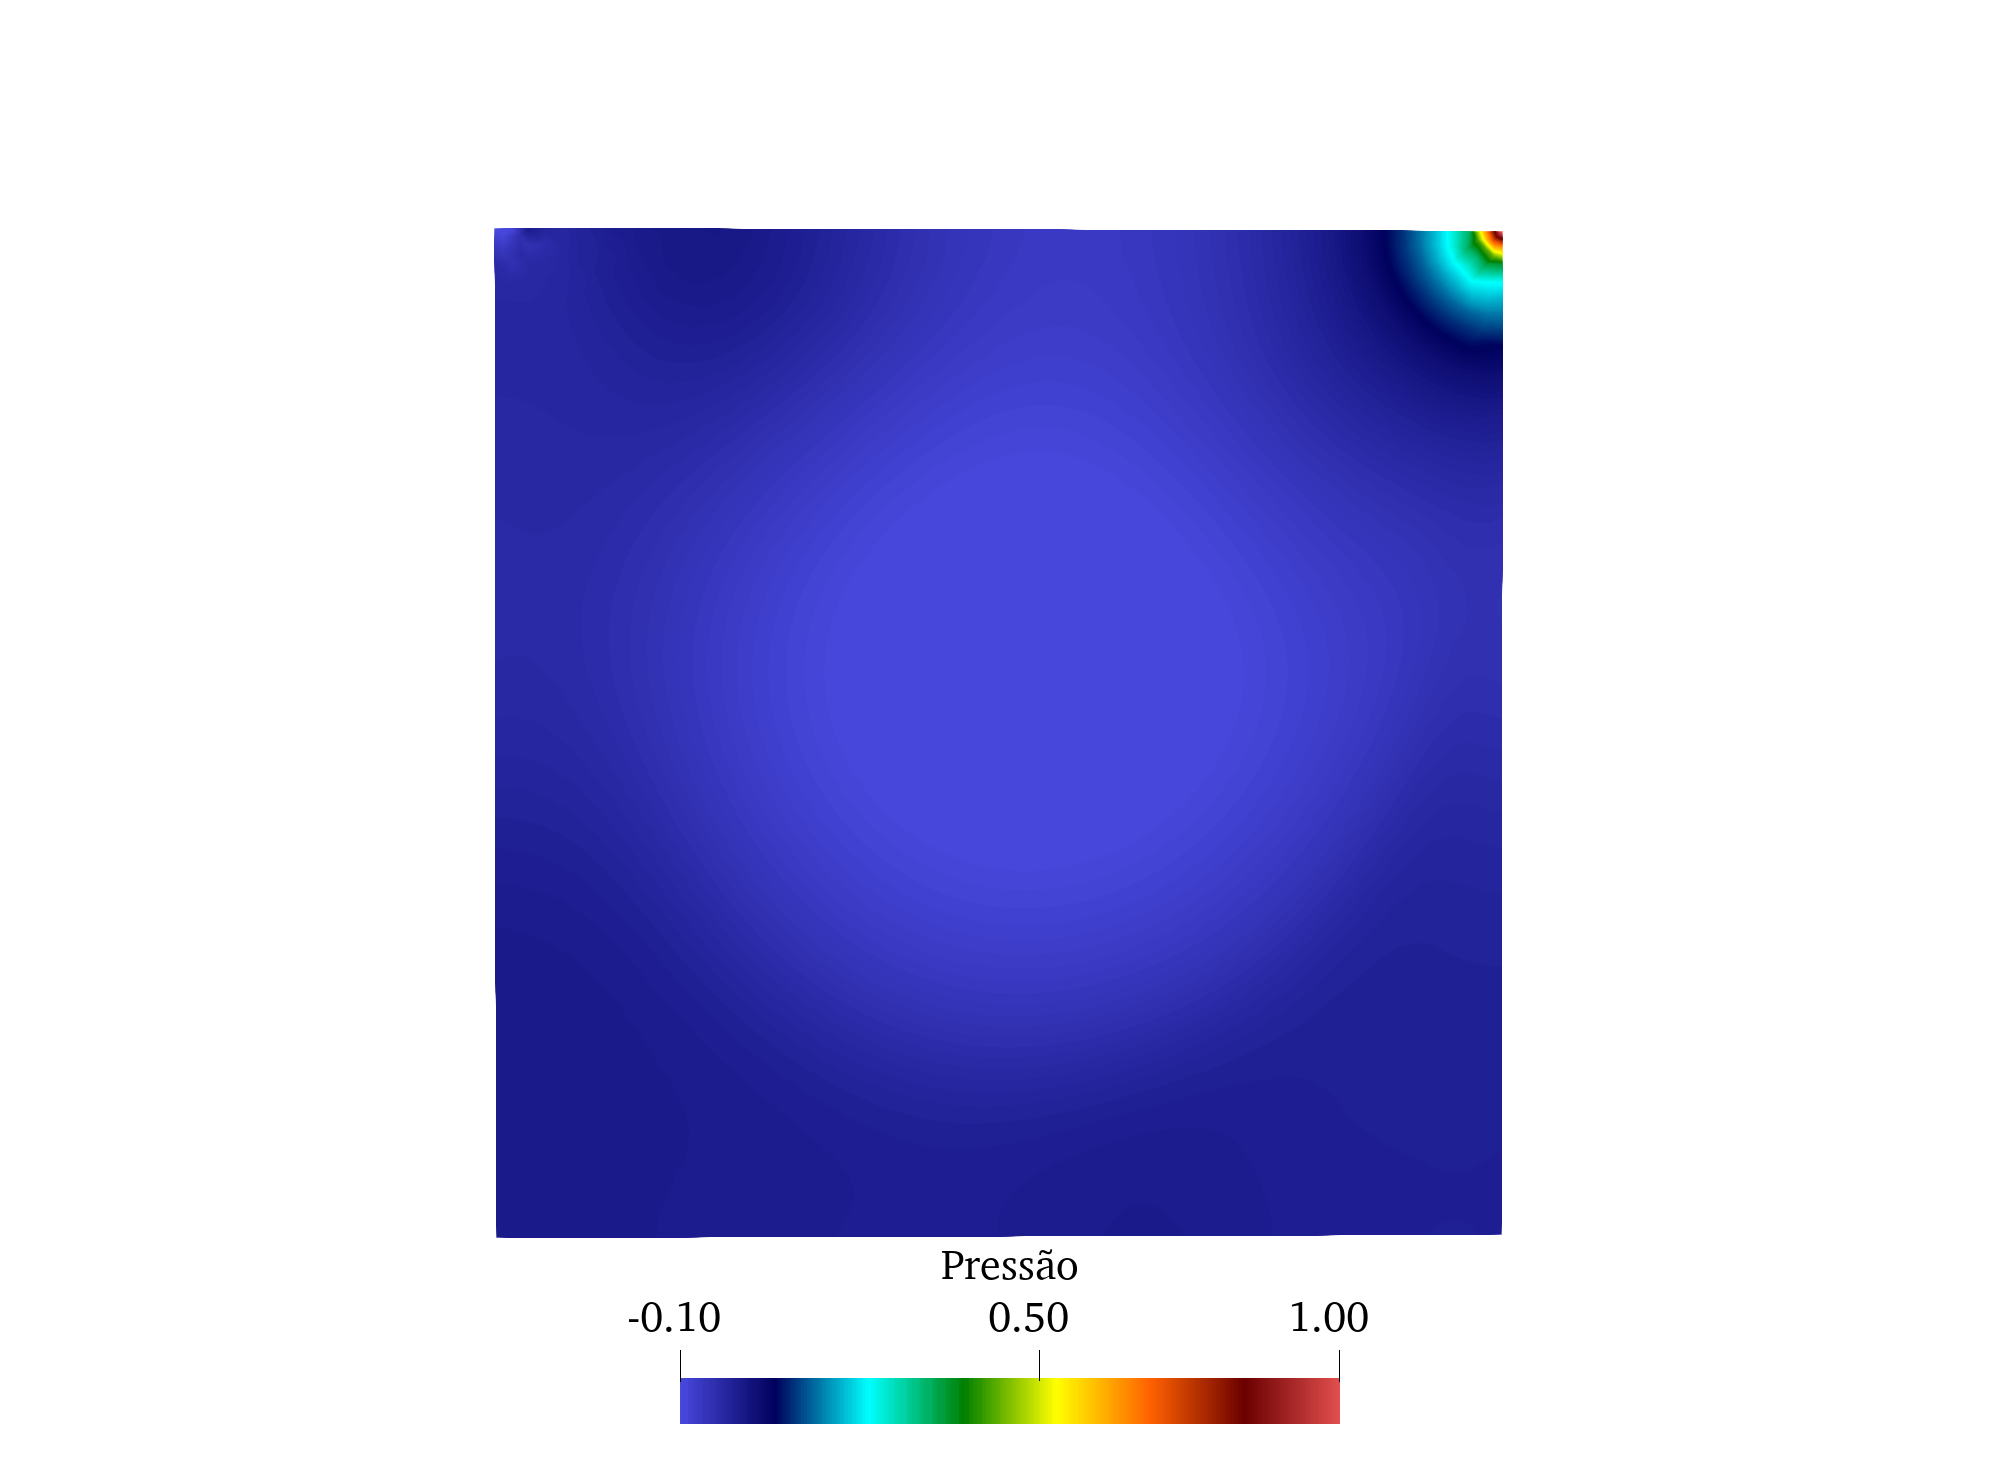
\includegraphics[scale=0.15,trim=15cm 0cm 15cm 7cm, clip=true]{Imagens/Cap2/pressao1000.png}} \\
	%	\subfloat[\label{fig:cavidade_g_Re10000}$Re$=10000.]{\includegraphics[scale=1.1,trim=0.55cm 0.5cm 0.3cm 0.2cm, clip=true]{Imagens/Cap2/cavidade_Re10000.eps}}\\
	\caption{Cavidade quadrada: campos de pressão. }
	\label{fig:cav3d-press}
\end{figure}


%
%\clearpage[e ]
%
%\textcolor{white}{ }


\end{document}
